\documentclass[12pt,a4paper]{book}
\usepackage{gtp}
\author{Compiled by Tanzanian Peace Corps Volunteers}
\title{General Education Practices for Teaching in Tanzania}
\setcounter{secnumdepth}{0}
\setcounter{tocdepth}{3}
\makeatletter
%%%%%%%%%%%%%%%%%%%%%%%%%%%%%% LyX specific LaTeX commands.
\special{papersize=\the\paperwidth,\the\paperheight}
%% Because html converters don't know tabularnewline
\providecommand{\tabularnewline}{\\}
%% A simple dot to overcome graphicx limitations
\newcommand{\lyxdot}{.}
\makeatother

\begin{document}

%Title Page
\begin{titlepage}
\begin{center}
\begin{huge}
\textbf{General Education Practices for\\[6pt]
Teaching in Tanzania}
\end{huge}
\end{center}
\vspace{1in}

\begin{center}
\setlength\fboxsep{0pt}
\setlength\fboxrule{2pt}
\fbox{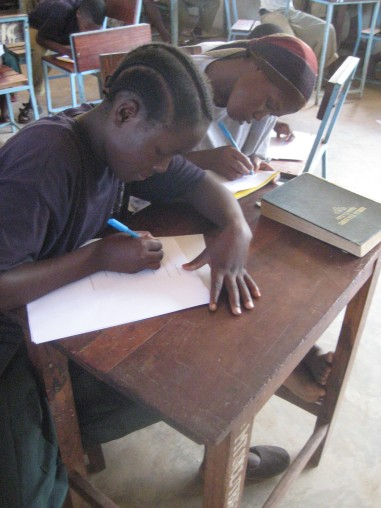
\includegraphics[scale=1]{./img/cover.jpg}}
\end{center}

\vfill
\begin{center}
\begin{Large}
Compiled by Peace Corps Volunteers\\
\end{Large}
\end{center}

\end{titlepage}

\tableofcontents
%Preface
\chapter*{Preface}
Peace Corps Education Volunteers are a diverse group of individuals. Some of us have been teaching for years while others are just starting the profession. This book will provide general education practices for teachers new to the trade as well as methods to teach your students in an interactive and engaging way. This book is filled with teaching ideas and successful solutions from Education Volunteers in this country. We hope you find this book useful and that you will contribute your own ideas to it in the future.

\vfill
\begin{center}
Main Contributors:\\
Claire Thomas\\
Carol Sevin\\
Ginny Morris\\
Colin Harari\\ 
Pat Stucke\\
Jeff Rodwell\\
Marilyn Bick\\
\end{center}


%Introduction to Teaching in Tanzania
\chapter{An Introduction to Teaching in Tanzania}
\section{A Good Teacher}
All of us have had teachers in the past that inspired us to learn.  Those teachers usually possess qualities such as kindness, a love for teaching, being lively and entertaining, motivation, having a passion and knowledge of subject, developing good rapport with the students, involving all students in teaching, correcting students without offending them, and knowing a student's weakness and strength.  These are qualities of a good teacher and ones we should strive for to make our lessons effective and inspirational.\\

A teacher has many roles in the classroom.  They are not just an instructor, but also as a manager, organizer, assessor, prompter, participant, tutor, facilitator, model, and observer.  A good teacher does not just lecture.  They manage students’ self learning, acting as a resource when necessary or participating alongside the student in learning.  Teachers are also role models for their students and can act as a counsellor if they observe something amiss in a student.\\

A teacher is a professional. Teaching is a noble profession.  Teachers develop the minds of future doctors, engineers, politicians, and parents.  Therefore, a teacher should always be a role model for their students. There are professional ethics to be followed by a teacher. Some practical points include:
\begin{itemize}
\item Being Punctual
\item Dressing Professionally
\item Preparing Lesson Plans
\item Respecting students 
\item Being a Leader
\item Being Honest
\end{itemize}

When we behave professionally and with the attitude of a teacher, our students and coworkers will respect us, regardless of age, gender, or nationality.  

\section{A Good Student}
Although it is unlikely that we will be blessed with all ``good'' students, we can encourage qualities of scholarship in our students.  A good learner is a student who is willing to listen and has a desire to experiment.  Good students are not afraid to ask questions and consider their own learning process.  By encouraging a desire to learn in our students, we can develop a more educated and thus more developed nation. \\

\begin{figure}[h!]
\centering
\setlength\fboxsep{0pt}
\setlength\fboxrule{2pt}
\fbox{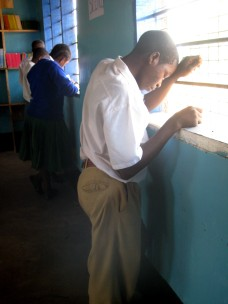
\includegraphics[scale=.08]{IMG_3697.JPG}} 
\end{figure}

When designing our lessons, we must consider our students' age, previous educational background, motivation, confidence, and language ability.  These may be different for each student.  As teachers we must be aware of these qualities and do our best to cater each lesson to the students’ abilities and needs.\\

Students learn in different ways.  Some learning types include: 
\begin{itemize}
\item verbal/linguistic
\item logical/mathematical
\item visual/spacial
\item musical/rhythmic
\item bodily/kinesthetic
\item interpersonal 
\item intrapersonal 
\end{itemize}



While teaching, we will face a variety of challenges that will prevent our students from learning.  Local culture or parents may not value education, discouraging children from studying or attending school.  Furthermore, students may may not relate education with work (or money), and therefore find it unimportant.  However, there are ways to motivate our students.  Such motivation for education could include future careers, study in other countries, improving the lives of themselves and their family, or bringing their country out of poverty.  

\section{Teaching in Tanzania}
Even for experienced teachers, teaching in Tanzania may prove to be a challenge.  The education system here is based on a British model that test students’ abilities with one final national examination.  Therefore, lessons tend to be focused on memorization rather than critical thinking.  \\

The Tanzanian education system is broken down into Primary, Secondary, and Tertiary education.  Primary education is compulsory, free, and begins around age 5 in Standard 1. In the mainland the medium of instruction is Kiswahili.  In Zanzibar, the students switch to English medium in Standard 5. Students will take a national exam in Standard 4 and again in Standard 7.  If they pass their Standard 7 exams (about 30 \% of students nationally), they will continue their education into Secondary School.  \\

Secondary education consists of Forms 1-6, with Forms 1-4 being Ordinary Level and Forms 5 and 6 being Advanced Level.  Students take a national exam (NECTA) in Form 2, but can continue their education whether they pass or fail.  Previously, students had to pass Form 2 exams to continue, but too many students were failing, so the government lifted this restriction.  In Form 4, students take another national exam.  If they pass in the top 3 Divisions, they may continue on to Advanced level.  If they get Division 4 or fail, they commonly find work as a primary school teacher, police officer, or attend vocational training schools.   Those who continue to Advanced Level will choose a three-course concentration for study.  In Form 6 they will take a final national exam on these three courses as well as General Studies.  If they do well, they will continue to University, if they do not, they usually become an Ordinary Level teacher or find private employment.\\

Tertiary Education is expanding rapidly in the country at the moment.  There are a wide variety of public and private universities, many of which offer Masters and even PhD programs.  Admittance into University is based solely on national examination scores and concentration in Advanced Level.  All applications are processed through an online application process.  University graduates may find work in the private sector, government or as instructors for Advanced Level.

\section{Common Challenges in a Tanzanian Classroom}
In any classroom a teacher will face common challenges like classroom management, diverse ability of students, and teaching with limited time and resources.  But Tanzanian education has its own unique challenges for teachers.  Because Tanzania was provided large amounts of foreign donor money to create schools, the education system grew explosively in the last 20 years.  Unfortunately, the Tanzanian government built secondary schools in each ward without securing resources or a teaching staff for those schools.  Thus, many schools volunteers teach at are under-resourced, both in materials and employees.  Because of limited staff, issues such as discipline, school management, and providing students with instruction for all subjects becomes a challenge.   Limited material resources affect both teaching aids in the classroom and retention of teachers.  Without electricity you cannot provide computer education or attract many new teachers.  However, there are ways to overcome these challenges which will be discussed further in Chapter 9 of this handbook.

\begin{center}
\setlength\fboxsep{0pt}
\setlength\fboxrule{2pt}
\fbox{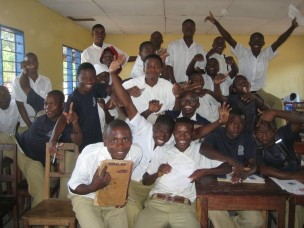
\includegraphics[scale=0.1]{IMG_3643.JPG}}
\end{center}

\section{Benefits of Teaching in Tanzania	}
Just as there are unique challenges to this education system, there are also opportunities that are not present in other parts of the globe.  First and foremost, it is much easier to make a large impact here than in other parts of the world where teachers are abundant. Additionally, you may be the only native English speaker your students have ever known, thus, providing them with a unique experience to learn the language and pass their examinations.  Because the limited staff, most volunteers are also much more involved in the administration of the school, providing a unique opportunity to learn more about the education system and overcome some challenges the school may be facing.  Because of the culture and close community, teachers may also become very close with students and their families, developing life long friendships.  As with any situation, teaching in Tanzania has its ups and its downs.  We hope through your Peace Corps experience you will learn to make the most of the challenges and savour the successes.  


%Making A Scheme Of Work
\chapter{Making a Scheme of Work}
Good teaching requires good preparation.  The first step in preparing to teach in Tanzania it to create a Scheme of Work. This document helps you to lay out your lessons for the year, so that you will be able to cover all topics in the syllabus in a timely manner with remaining time to review.  Many people may tell you to copy the syllabus as the scheme of work, but this is a waste of time and in no way beneficial to you.  Instead, take a day and lay out your plans for the year.   Cater your Scheme of Work to your needs and the needs of your students. Below is a sample of the heading columns in a scheme of work. Remember, you should edit this document, adding or subtracting columns, in a way that makes sense to you.

\begin{flushleft}
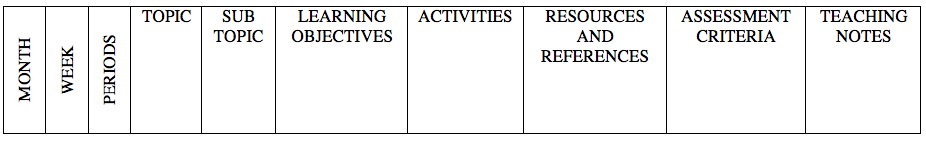
\includegraphics[scale=.4]{./img/picture-1.png} 
\end{flushleft}


\section{How to Begin}
First, choose the topic in your subject you would like to begin the year with.  You may decide to follow the syllabus and teach the topics in the order the Ministry has outlined or you may decide to create your own order, choosing to teach the most important or relevant topic first.  Then, list the remaining topics in that subject and the order in which you would like to teach them.  Next, list the subtopics in each of those topics, again changing the order of the subtopics as you see fit.\\

\pagebreak
\begin{flushleft}
\begin{small}
For Example:\\
Biology Form IV\\
\textbf{1.0 Classification of Living Things\\}
1.1 Kingdom Animalia\\
1.1.1 Phylum Platyhelinthe\\
1.1.2 Phylum Aschelminthes (Nematoda)\\
1.1.3 Phylum Annelida\\
1.1.4 Phylum Arthropoda\\
1.1.5 Phylum Chordata\\
\textbf{2.0 Growth\\}
2.1 Concept of Growth\\
2.2 Mitosis and Growth\\
2.3 Growth and Development in Human Beings\\
2.4 Growth in Flowering Plants\\
\textbf{3.0 Genetics\\}
3.1 Concept of Genetics\\
3.2 Genetic Materials\\
3.3 Concept of Inheritance\\
3.3.2 Mendelian Inheritance\\
3.3.3 Non-Mendelian Inheritance\\
3.4 Sex Determination and Inheritance\\
3.5 Variation among Organisms\\
3.6 Genetic Disorders \\
3.7 Application of Genetics\\
\textbf{4.0 Evolution\\}
4.1 Concept of Organic Evolution\\
4.2 Theories of the Origin of Life\\
4.3 Theories of Organic Evolution\\
4.4 Evidence of Organic Evolution\\
\textbf{5.0 HIV, AIDS, and STIs\\}
5.1 Relationship between HIV, AIDs, and STIs\\
5.2 Management and Control of HIV/AIDs and STIs\\
5.3 Counseling and Voluntary Testing \\
\end{small}
\end{flushleft}

\section{Time Frame}
Now consider the amount of time it will take you to teach each of these topics and their subtopics. Use the syllabus while you are doing this.  Consider what the objectives are for each subtopic and how long it will take you to accomplish these objectives.  Consider the student background education as well.  For example, if you are teaching a topic in physics, maybe you want to add a period to review the mathematics required.  You may use the timetable in the syllabus as a guide, but you know your students better than the average time allotted by the Ministry of Education.  Each period is allocated a different amount of time per week.  Refer to the table below to determine how many periods a week your subject is allocated.\\

\begin{center}

\begin{tabular}{|c|c|c|}
\hline \rule[-2ex]{0pt}{5.5ex} Subject & Form & Periods per Week \\ 
\hline \rule[-2ex]{0pt}{5.5ex} Biology & 1,2 & 3 \\ 
\hline \rule[-2ex]{0pt}{5.5ex} Biology & 3,4 & 4 \\ 
\hline \rule[-2ex]{0pt}{5.5ex} Biology & 5,6 & 10 \\ 
\hline \rule[-2ex]{0pt}{5.5ex} Chemistry & 1,2 & 3 \\ 
\hline \rule[-2ex]{0pt}{5.5ex} Chemistry & 3,4  & 4 \\ 
\hline \rule[-2ex]{0pt}{5.5ex} Chemistry & 5,6 & 10 \\ 
\hline \rule[-2ex]{0pt}{5.5ex} Physics & 1,2 & 3 \\ 
\hline \rule[-2ex]{0pt}{5.5ex} Physics & 3,4 & 4 \\ 
\hline \rule[-2ex]{0pt}{5.5ex} Physics & 5,6 & 10 \\ 
\hline \rule[-2ex]{0pt}{5.5ex} Mathematics & 1-4 & 6 \\ 
\hline \rule[-2ex]{0pt}{5.5ex} Mathematics & 5,6  & 10 \\ 
\hline \rule[-2ex]{0pt}{5.5ex} English & 1-4 & 6 \\ 
\hline 
\end{tabular} 

\end{center}
Therefore, your Scheme of Work should now look something like this:

\begin{flushleft}
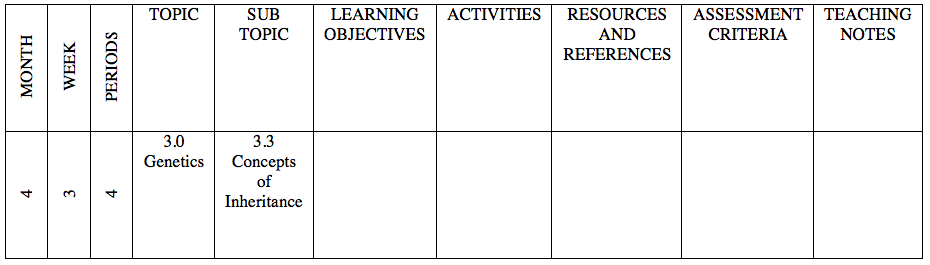
\includegraphics[scale=.4]{./img/picture-2.png} 
\end{flushleft}

\section{Learning Objectives}
These are taken from the syllabus and are the one thing you can copy and paste directly.  Read each one of the corresponding subtopics and be sure the amount of time you have allocated for that subtopic is sufficient to meet these objectives.  You can reword or add objectives to this list as you see fit.

\section{Activities}
Now comes the hard work: brainstorming for future lessons.  This will be a great reference when it comes time to write your lesson plans.  In this column, list possible activities for you and your students to complete during class to meet the learning objectives for the subtopic.  Be creative here.  These ideas are not set in stone, but rather possibilities for interactive teaching.  This column may be broken into two columns as well; Teacher's Activities and Students' Activities. It is up to your discretion whether you would like to combine the two or keep them separate. At this point, you Scheme of Work should appear as follows:

\begin{flushleft}
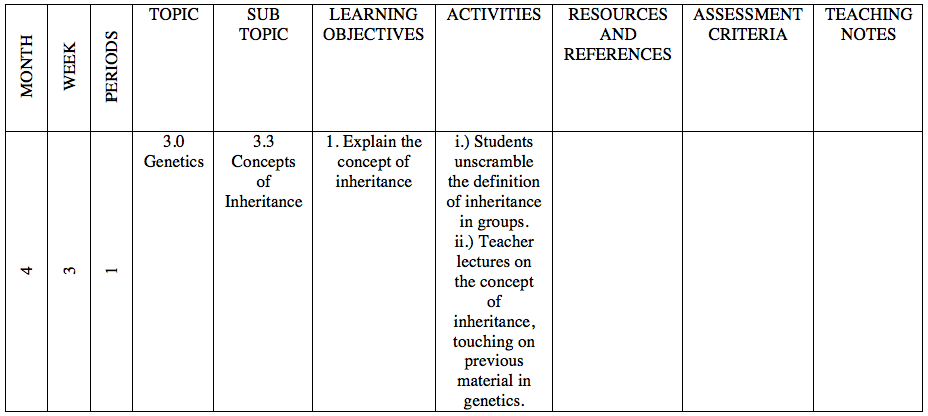
\includegraphics[scale=.4]{./img/picture-3.png} 
\end{flushleft}

\section{Resources and References / Teaching Aids}
Review your activities in the previous column.  What materials or academic references do you need to make these activities a success?  You can include websites or reference books and their page numbers here, as well as any resources you might need to complete labs or games.

\section{Assessment Criteria}
This column is one of the most beneficial in the future when you are creating quizzes, assignments, and tests.  How will you know if your students have in fact reached the objectives for that subtopic?  This assessment criteria can be phrased in the form of a question or statement, but should be specific and reflect your lessons.  Consider the types of questions asked on NECTA, rather than referring to the very general assessment criteria in the syllabus.\\
Some examples: 
\begin{itemize}
\item Students can name the three states of matter and give an example of each
\item Students can calculate the volume of a cylinder from a word problem
\item Students will be able to list 5 advantages and 5 disadvantages of Kingdom Fungi
\end{itemize}
  

\section{Teaching Notes or Remarks}
This column will be left blank for observation or changes you may have in the future.  If a subtopic took longer to teach than you allocated, note this for next year.  It is possible you may want to change the topic order, or you found certain activities that worked well or not at all.  These will be noted in the Teaching Notes column after you have taught those lessons.  
Thus your final Scheme of Work will appear as follows:

\begin{flushleft}
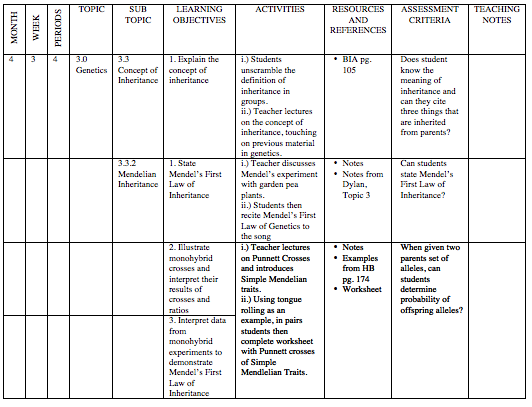
\includegraphics[scale=.7]{./img/picture-4.png} 
\end{flushleft}

Creating a Scheme of Work may seem tedious or bureaucratic but it makes creating lesson plans and tests much easier.  A good Scheme of Work will keep your instruction organized and ensure that you have covered all topics and objectives with your students.  The Ministry of Education also requires it.   Try creating a document that is actually useful to you, rather than spending hours copying one that is not.

%Lesson Planning
\chapter{Lesson Planning}
There are a variety of different types of lesson plan formats that volunteers can use in teaching. The most important thing is that teachers enter the classroom with a lesson plan. Often times, teachers come to class with only their lecture notes, making the lesson unengaging for students, especially those who are not fluent in English. Lessons plans allow us to create interactive lessons that involve the class as a whole and get students interested in the learning material. This develops those qualities of a good learner, as students now want to learn and ask questions. These are the key components to any lesson plan:

\begin{itemize}
\item It must engage or interest the student
\item It should be relevant or be applicable to the students' lives
\item It should encourage the students to think and make their own conclusions
\item It should allow the student to acquire new knowledge
\item It should include lesson notes which are in simple English and written in full sentences
\item It should include the amount of time required for each portion of the lesson and the materials needed
\item It should include a formal or informal assessment of what students have learned
\item It should have notes to improve the lesson in the future
\end{itemize}

\begin{figure}[h!]
\centering
\setlength\fboxsep{0pt}
\setlength\fboxrule{2pt}
\fbox{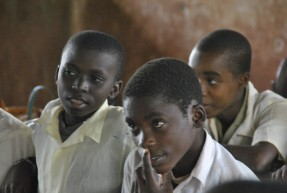
\includegraphics[scale=.09]{./img/DSC1801.JPG}} 
\end{figure}

In the following pages you will find three types of lesson plans, and an explanation of each.  You can choose one of the following formats or make your own.  Remember, this is your guide for the class and is extremely important to ensure you are teaching engaging and useful lessons for the students, rather than just lecturing at them and hoping they absorb the material.  Further interactive teaching ideas can be found in Chapter 9, Teaching Topics and Ideas.


\newpage

\begin{center}
\section{Engage, Acquire, Practice, Reflect}
\textbf{Developed by PCVs} \\
\end{center}

\begin{flushleft}
First, \textbf{Engage} your students \\
Then, encourage them to \textbf{Acquire} knowledge \\
Third, allow them to \textbf{Practice} what they have learned \\
Final, \textbf{Reflect} together what has been taught and understood \\
\end{flushleft}

\subsection{Activities to Help Students Engage:}
Engage your students in the first 5-10 minutes of class to get them thinking about the topic at hand.
\begin{itemize}
 \item Review Questions
 \item Demonstration
 \item Hands-on experiments
 \item Definition Scramble
 \item Race (who can draw diagram the quickest, answer problem)
 \item Games (list the most prime numbers in 3 minutes)
 \item Puzzles
 \item Motivating questions 
 \item Brainstorming
\end{itemize}

\subsection{Activities to Help Students Aquire Knowledge:}
Teach your students material in a way that is interactive and fun.  
\begin{itemize}
 \item Interactive Lecturing
 \item Group Work
 \item Hands On Experiments
 \item Projects
\end{itemize}

\subsection{Activities to Help Students Practice and Reflect:}
At the end of class, evaluate whether your students have learned the material and understand its importance.
\begin{itemize}
 \item Scavenger Hunts
 \item Review games
 \item Oral Quizzing
 \item Debate
 \item Essays
 \item Homework
 \item Tests and quizzes
 \item ``Today I Learned...''
\end{itemize}

\newpage
\begin{center}
\textbf{Engage, Acquire, Practice, Reflect\\ \textit{Sample Lesson Plan}}\\
\end{center}
\textbf{\textit{ }}\\

\begin{center}
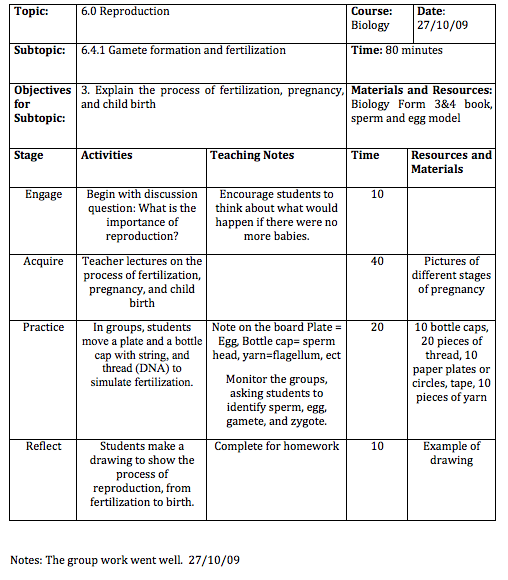
\includegraphics[scale=.8]{./img/picture-5.png} 
\end{center}

\newpage
\begin{center}
\section{I Do, You Do, We Do}
\textbf{Developed by Ellen Levy}\\
\end{center}

Scaffolded instruction, sometimes referred to as ``I do it, we do it, you do it'' moves classroom instruction from teacher-centered, wholegroup delivery to student-centered collaboration and independent practice.  This method is used in the training of Teach for America Volunteers and was created by Ellen Levy. \\

\begin{center}
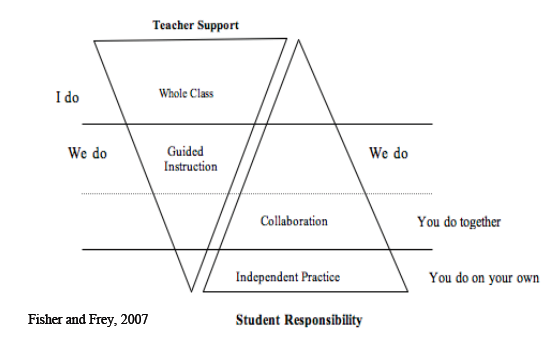
\includegraphics[scale=.5]{./img/i-do-you-do-triangle.png} 
\end{center}

Taken as a whole, the triangles represent the mentoring relationship and two-way interaction between the teacher and student. At the beginning of a lesson or when new material is being introduced, the teacher has a prominent role in the delivery of the content. This is the ``I do'' phase. But as the student acquires the new information and skills, the responsibility of learning shifts from teacher-directed instruction to student-processing activities. In the ``We do'' phase of learning, the teacher continues to model, question, prompt and cue students; but as students move into the ``You do'' phases, they rely more on themselves and less on the teacher to complete the learning task.

\begin{center}
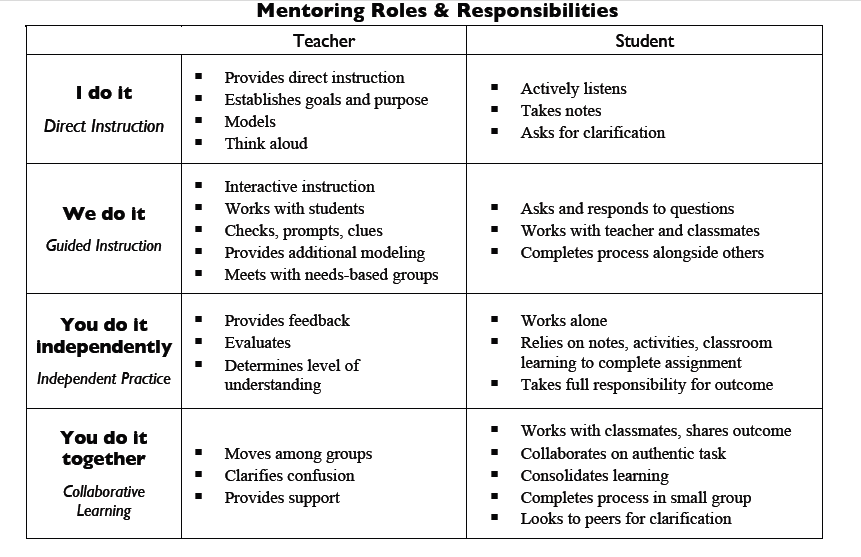
\includegraphics[scale=.5]{./img/i-do-you-do.png} 
\end{center}

\newpage
\begin{center}
\textbf{I do, We do, You do }\\
\textit{Sample Lesson Plan}
\end{center}

\begin{center}
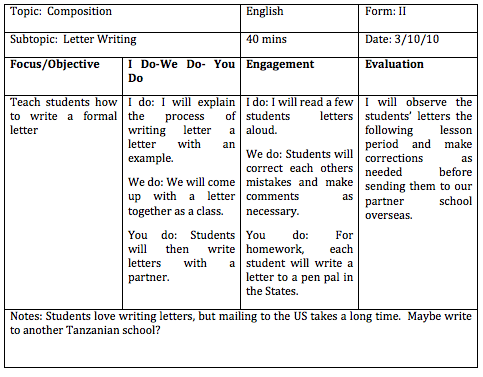
\includegraphics[scale=.8]{./img/picture-6.png} 
\end{center}

\newpage
\begin{center}
\section{4MAT}
\textbf{Developed by Bernice McCarthy}\\
\end{center}


4MAT uses the basis of learning profiles and brain modality to develop a 12-step process within a 4-quadrant cycle for learning a given unit or lesson.  This strategy allows you to actively seek to engage every learner through a variety of tactics designed to constantly apply and direct their learning to real-world applications.


\begin{center}
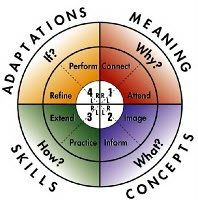
\includegraphics[scale=1]{./img/mat-wheel.jpg} 
\end{center}

\begin{flushleft}
\textbf{Why?} (Quadrant 1 on the wheel)
Answering this question establishes relationships with the content, and personal, meaningful connections based on previous experience.\\

\textbf{What?} (Quadrant 2 on the wheel)
Answering this question allows the student to connect, comprehend, organize, classify and clarify the knowledge.\\

\textbf{How?} (Quadrant 3 on the wheel)
Answering this question allows the student to practice, experiment and get hands-on with the information being presented.\\

\textbf{What If?} (Quadrant 4 on the wheel)
This is where the students will modify, refocus, summarize and ultimately perform the knowledge they have acquired in a real-world context that aids in answering the essential question for the unit or lesson.\\

\end{flushleft}

\newpage
\begin{center}
\textbf{4MAT }\\
\textit{Sample Lesson Plan}
\end{center}

\begin{center}
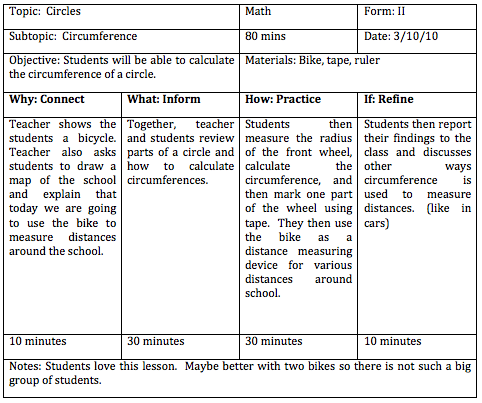
\includegraphics[scale=.8]{./img/picture-7.png} 
\end{center}
%Interactive Teaching
\chapter{Interactive Teaching}
As we have seen in our sample lesson plans, there are times when a teacher will be lecturing.  However, lecturing to students for whom English is a second or even third language needs to be engaging and visual.  We can not use the same lecture style we were raised on. We knew English and also how to take notes while listening. Instead, we should use interactive teaching techniques to keep our students interested, help them  understand, and improve their English. \\

Interactive lecturing means that although the teacher may at points be the lead speaker, students are still answering questions, asking questions, and focused on the topic at hand.\\

The following suggestions may be helpful in practicing Interactive Teaching:

\section{Learn definitions in a fun way}
Instead of just reading a definition aloud and hoping students will memorize it, help them commit it to memory.  Try reading the definition one student, one word at a time.  This involves all students in the class, makes them speak up, and keeps them paying attention.  Additionally, you can have students break into groups and race to unscramble a definition that has been written word by word on manila paper.\\

\section{Ask Questions}
By asking our students questions, we can access their understanding, build their confidence, and get them speaking English. Try these techniques to get your students answering questions:
\begin{itemize}
\item Start the class each day with review questions from the lesson before to get students' mind on the topic at hand and build their confidence before they enter a new subject.
\item Once the notes are written on the board, ask students questions from the notes, like ``Who can tell me, what are the three types of locomotion?'' rather than students or instructor just reading the notes allowed.
\item Ask questions that call for a choral responses.
\item When a student answers a question, ask the rest of the class if they are correct or incorrect.
\item Have one student answer a question, then have them ask another student a different question.
\item Have students come to the front and face the class to answer questions.
\item Trying using a question ball.
\item Write a question on the board and have students come to the board to answer, then they write a question and have another student answer it.
\end{itemize}

\section{Give Participation Points}
To encourage students answering questions and reading aloud, give a point in the top hand corner of the board every time someone volunteers.   This works very well for girls empowerment and is discussed more in Chapter 8.\\

\section{Be Visual}
When teaching in a foreign language, we should try to be as visual as possible.  Use pictures and examples whenever possible.  If you are teaching about classification, draw the organisms and quiz students.  Common accidents in the chemistry lab could also be drawn and used to teach students the hazards and new English vocabulary.   Teach students shapes by drawing them rather than their Kiswahili name.\\ 

\section{Be Active}
Some topics may be difficult for students to grasp, especially while learning in a new language.  Act out things and get the kids involved whenever possible.  If you are talking about hearing, ask students to touch their ears.  When describing a lever, move your arm.  If you are discussing temperature regulation, have students act like they are in a hot/cold environment.\\  

\begin{figure}[h!]
\centering
\setlength\fboxsep{0pt}
\setlength\fboxrule{2pt}
\fbox{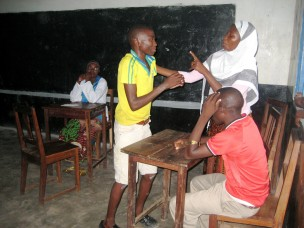
\includegraphics[scale=0.3]{./img/IMG_5127.JPG}} 
\caption{Students acting out the negative effects of Drug Abuse}
\end{figure}

\section{Repeat Difficult Words}
When you are lecturing, note words that might be difficult to say and have the students repeat the word out loud.  Its wakes them up, they practice pronunciation, and they love doing it.\\
Additionally, you can have students spell out the pronunciation of difficult words.

\section{Group Work}
Group work facilitates learning.  Teachers need to organize small groups of students and then teach the students how to work together and help each other learn. All students should be writing and active in the learning, not just one student.  The teacher should guide students to stay on task and move around the room to observe students' progress and give praise. If a group is working too slowly, another student can come to that group to help teach.  When groups are finished, questions answered are (or work done
is) shared and discussed as a class.\\

Questions can also be written on card paper and handed to small groups to be discussed. They can then be passed on to another group.  These cards can also be used like a scavenger hunt.  Groups get one question and when they answer it correctly, they get another question to answer.  The first group to answer all their questions wins.

\section{Critical Thinking}
Critical thinking is key to each lesson.  New material is not given to memorize but to understand and be used. Critical thinking is the process of analyzing, comparing, processing, and using new information. When teaching, ask your students critical thinking questions from the material you presented.  Have students present debates on topics when possible.  Ask students to make a list of scientific questions they have about a topic and then discuss them as a group.

\section{Projects}
Giving students projects allows the students to teach themselves and determine what information is important. Using your school's library, teach students how to use the table of contents and index to find information. Once they create their project, have them present and teach other students. You can also bind the project papers together into a book (1000/=) and put in the library for future use and to create pride in students' work.

%Classroom Management
\chapter{Classroom Management}
Good classroom management is essential to creating a learning environment for your students and allowing you to love your job.  In order for our students to feel comfortable learning, we need to establish an environment that is conducive to engaging all types of students.  The teacher as a guide and facilitator helps to establish a learning environment of collaboration and cooperation.

\section{Manage your space}
In most schools, teachers will be entering a classroom for each form, rather than having their own space like in the United States.  This does not mean you can't arrange the classroom or make it your own during your class period.   

\begin{itemize}
 \item Set up classroom rules with your students. Usually 5 positive rules are sufficient. For example: We will not laugh at other students, Students will be prepared for class, Students will complete assignment, Students will be on time.  Have consequences clearly defined if these rules are broken and stick to them.  
 \item Walk around the classroom while lecturing to monitor behavior and understanding in your students.  
 \item Use non-verbal signs with students to indicate being quiet or going to the bathroom.
 \item Divide your board into 3 or 4 sections at the beginning of class.  Use 2 or 3 for notes, leaving the final space open for pictures, examples, or vocabulary building. Make sure to write the date and subject in the top right corner of the board.
 \item Do not try to talk while students are still writing notes. Instead, have students put their pens down or in their pockets when you want them to listen, so they can not write while you teach.
 \item Greet your students when you enter class and thank them for a good lesson at the end of class.
 \item Teach subject content on the first day of school.
 \item Have students create posters to hang around the class to help with their English or other subject matter.  Create a ``clothes line'' and hang the posters with clothes pins so they can easily be removed on test days.
\end{itemize}

\section{Know your students}
It is important  that we know our students, both to encourage them in the classroom and to know when they may need our help in other areas of life.  

\begin{itemize}
 \item Learn students names.  A good English exercise for this is having students stand in a circle.  The student says ``This is (the name of the person to the left). My name is \_\_\_\_'' and continue around the circle in that manner. An occasional roll call, being observant
when handing back papers, and mentally registering names while
students are writing tests.  Students will be surprised and proud if
you call them by name unexpectedly.
 \item Set up office hours.
 \item Have meetings with students when you hand back tests to talk about strengths and weaknesses. 
 \item Local and national culture will greatly influence your students behavior.  Be sensitive to this fact.
\end{itemize}

\section{Expect the best}
We need to have high expectations for our students and believe they can succeed.  If we have high expectations for our students, they will try to meet them. 

\begin{itemize}
 \item Say the learning objective at the beginning of the class.  ``Today, we are going to learn how to write an essay.   By the end of class, you will be able to write an essay on HIV.''
 \item Make sure your students are writing notes and not working on other subjects during your period.  
 \item Call on students who may have the answer but are afraid to speak up.  Give homework and have students share in the following class.  
 \item Allow students to teach class or serve as an example when they do an assignment especially well.
\end{itemize}

\section{Establish Procedure}

Create routine in the classroom so students know what to expect.  This saves time and your voice from having to repeat instructions.   Consider things like how to begin class, bathroom breaks, group work, writing notes, listening to instruction, answering questions, and students who may be off task or unprepared. Use the following classroom procedures or create your own. 

\begin{itemize}
 \item Greet students and ask them to sit in their seats.
 \item Everyone gets out the materials they need for class.
 \item When the teacher is writing, students are writing.
 \item When the teacher says ``Pens down", students are listening.
 \item To use the bathroom, a student must raise their hand with fingers crossed.  Teacher will nod to give permission.  They will re-enter without interrupting class.
 \item When answering questions, students will stand straight and speak loudly and clearly.
 \item Teacher will walk around the room to monitor class progress and understanding.  Students not on task or unprepared for class will be asked to leave.
 \item At the end of class, students will ask questions and write down homework assignment.
\end{itemize}

\section{Give praise}
Many of our students are coming from homes where they may receive little vocal praise or affirmation.  Be sure to reward good behavior and work ethic.

\begin{itemize}
 \item Show off students work in the school library, class, or school display board.
 \item Use positive words of praise.  (Good, Great, Awesome, Good Job, Very cool, Well Done)
 \item Allow getting the wrong answer to be ok. ``Good idea, but I asked \_\_\_\_\_. Can you try again?'' ``Think, are you sure that is correct?''  
 \item Reward high scoring students and most improved students with pencils, stickers, or candy.
\end{itemize}

\section{Disruptive Behavior}
Hopefully, you will establish a classroom that will have few discipline problems.  However, there are times when students may break rules.  The following are ideas for preventing problem behavior and what to do when it may occur.

\begin{itemize}
 \item Establish working rules and consequences.
 \item Establish a relationship with students based on respect.
 \item Give praise for appropriate behavior.
 \item Encourage students to work together.
 \item Involve parents in their child's education and behavior.
\end{itemize}

Unfortunately, many of our schools are understaffed, creating meaningful and behavior changing consequences for misbehavior can be difficult.  Remember, punishment and consequences are two different things.  We may not hit our students, but having them kneel in the front of class or do pushups doesn't teach them why what they did is wrong.\\  

Try the following consequences for common problem behavior:
\begin{itemize}
 \item Put on a serious face and stare at the student until they become quiet. Ask them what they are doing.
 \item Ask a misbehaving student what they are doing and what they should be doing right now.
 \item When a student asks to be forgiven tell them you forgive them, but because they have broken a rule, they will face the consequences.
 \item Cut off a student if they continue to argue. ''We will discuss this at another time, now you need to \_\_\_\_"
\end{itemize}

There are times when you may be one of two teachers at your school.  During these times it may be very difficult to execute the above-mentioned discipline measures.  Do not let other students learning suffer because one student's poor decisions.  If needed, remove the disruptive student from class and deal with them later.  Show your students that it is a privilege to study in school and one they should not take for granted.


\section{Get back your classroom}

Sometimes we can have a rough day in class that can make us doubt ourselves, which affects our teaching and classroom management.  If you feel that student behavior is slipping, follow these guidelines to get back on track:

\begin{itemize}
 \item Relax and get a good night's sleep
 \item Review the rules you set for the class.  Why are the students violating them?  Do the students understand them?
 \item When you enter the classroom, be firm but positive.
 \item Review the rules again with your students, clearly stating the consequences if broken.  Be confident.  You are a good teacher and deserve to be treated as such.
 \item Be firm and consistent in enforcing the rules.  Have a zero-tolerance policy for rule breaking.
 \item Seek advice from a counterpart or another Peace Corps teacher. Remember, you are not alone! 
\end{itemize}

%Evaluating and Testing
\chapter{Evaluating and Testing}
Now that we have taught our interactive lessons, we need to be sure our students have actually obtained knowledge.  We can do this through formal and informal evaluations.\\
  
Informal evaluations can usually be done during or at the end of class, to ensure everyone is on the same page.  Examples of informal evaluations would be:

\begin{itemize}
 \item Quizzing students verbally
 \item Competition between boys and girls to answer questions
 \item Using flashcards to test understanding
 \item Doing games or races with students to find the answer
\end{itemize}

Informal evaluation is useful because you can quickly see whether students have understood the information presented and if certain topics need to be taught again.  However, it is more difficult monitoring long-term progress of individual students or pin pointing issues the students may be struggling with.\\

Formal evaluations are homework, tests, and quizzes which would receive a grade.  These grades can be tracked overtime, and used as an indicator of student progress.  However, tests usually come at the end of a topic, and may be too late for a teacher to re-teach the topic if it was found completely misunderstood by students. To best serve our needs, examinations should:

\begin{itemize}
 \item Follow the NECTA format
 \item Find a balance between the difficulty of NECTA exams and what is taught in class
 \item Have some questions from previous NECTA  exams on the test
 \item Test on the material you have provided your students
\end{itemize}

When you get tired of students failing, test their collective knowledge with a group test.  Write one question on the board at a time and select a student at random to answer it.  All students get the collective grade.  May encourage your stronger students to help the ones who don't study.  To avoid cheating, make sure the class is silent and have the student come to the board before you write the question.

We can also evaluate our own work.  We can ask students to evaluate our course through a questionnaire or discussion.  This promotes genuine interaction, develops a much greater awareness among students of what is happening in the classroom, and helps you understand better how they react to your teaching. See the section on Teacher Evaluation later in this chapter.

\section{Test Content}

We hope to teach our students a combination of knowledge and application of the newly learned information.  By using Bloom's cognitive levels, we can evaluate the outcomes of our instruction.

\begin{center}
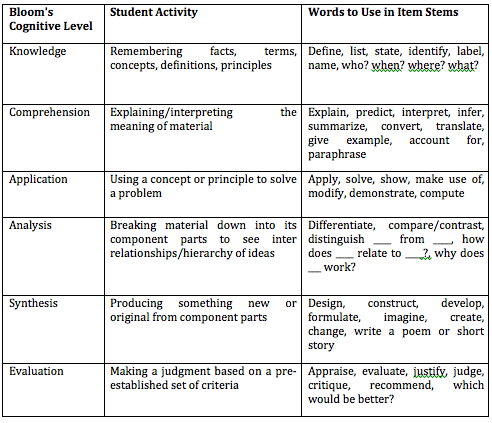
\includegraphics[scale=1]{./img/picture-8.png} 
\end{center}

When writing a test we also want to ensure that the number of questions we include on that test represents the amount of time we spent teaching those concepts in class.  The easiest way to ensure a representative sample of content and cognitive objectives on the test is to prepare a table of specifications. This table lists the content topics on one dimension and the cognitive skills on the other. We want to include content and skills in the same proportion as they were stressed during instruction.\\

\begin{figure}[h!]
\begin{center}
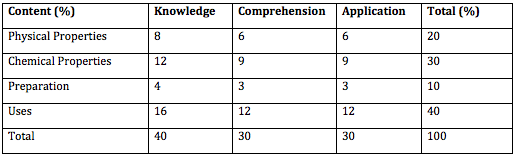
\includegraphics[scale=1]{./img/picture-9.png}
\caption{Table of Specification for a Chemistry Unit Test on Oxygen}
\end{center}
\end{figure}

This table indicates the content topics, the objectives to be covered and the proportion of the test that will be devoted to each. Evidently, more class time was spent on the uses of oxygen because 40\% of the test questions deal with uses compared with only 10\% on preparation. The column totals indicate that 40\% of the items will be written at the knowledge level with the remaining divided equally between comprehension and application. Using the percentages assigned to each cell, we can write the appropriate number of items. For example, because 20\% of the test is to cover physical properties and 30\% is to be application, then 6\% of the total test would measure the ability to apply knowledge about oxygen's physical properties to new situations.\\

Using a table of specifications aligns test content with instruction content, ensuring content validity of the test.  Using a table of specification also helps an instructor avoid one of the most common mistakes in classroom tests, namely writing all the items at the knowledge level.

\section{Format}

As mentioned earlier, we want to ensure that our test format reflects the style of questions that will be on the NECTA exam.  Most NECTA exams contain the following format:

\begin{enumerate}
 \item Form II
 \begin{enumerate}
  \item Multiple Choice, Matching, and True and False
  \item Short Answer
  \item Guided Essay
 \end{enumerate}
 \item Form IV
  \begin{enumerate}
  \item Multiple Choice and Matching
  \item Short Answer
  \item Essay
 \end{enumerate}
\end{enumerate}

Therefore, our examinations should include similar style of questions so that our students are not seeing these types of questions for the first time when they sit for the NECTA exam.   We can prepare questions in advance from previous NECTA exams by creating a question bank, sorted by form and topic.  This helps us in two ways: (1) it shows what topics are most commonly asked on NECTA exams, (2) it allows teachers to quickly find questions from NECTA to use on their tests. 

\section{How to Write a Better Test}

As noted before, assessing and evaluating students learning process is essential for the student and teacher in order to improve.  Therefore, it is important that we create tests that assess our students knowledge properly and encourage them to study. Below are a list of common problems when writing tests:

\begin{enumerate}
 \item Tests include too many questions measuring only knowledge of facts. One of the most common complaints from students is that the test content did not reflect the material discussed in class or what the professor seemed to indicate was most important. This may happen because knowledge questions are the easiest to write.
 \item Too little feedback is provided. If a test is to be a learning experience, students must be provided with prompt feedback about which of their answers were correct and which were incorrect.
 \item The questions are often ambiguous and unclear.  Ambiguous questions often result when instructors put off writing test questions until the last minute. Careful editing and an independent review of the test items can help to minimize this problem.
 \item The tests are too short to provide an adequate sample of the body of content to be covered. Short tests are not fair to students.
 \item The number of exams is insufficient to provide a good sample to students' attainment of the knowledge and skills the course is trying to develop. 
\end{enumerate}

\section{Grading}

Give partial points for correct answers, especially in Mathematics or calculation questions.  Give full points for correct answers, half points for correct procedure, but poor calculations, and no points if no attempt was made.  Write a making scheme that outlines the marks awarded for each question at the time of writing the test.

\begin{figure}[h!]
\begin{center}
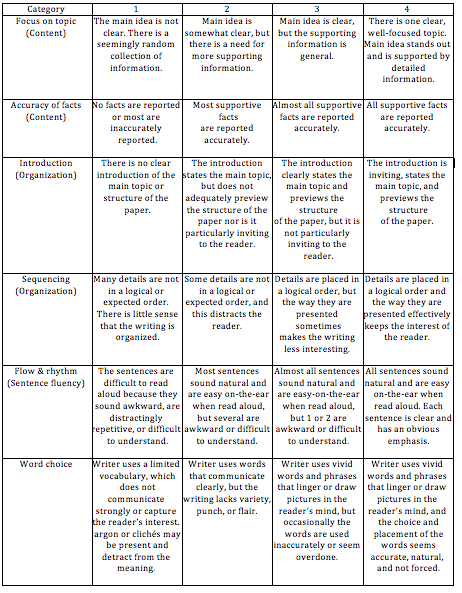
\includegraphics[scale=1]{./img/picture-10.png} 
\caption{Rubric for Grading an Essay}
\end{center}
\end{figure}

When grading essays or other writing, create a rubric.  Give a number of points for organization/format, content, and grammar and spelling.  For example, on a 20 point essay, 5 points are allotted to format, with 1 point being poor and 5 being excellent.  10 points are awarded to content, each point made in the essay 1 point and additional 2 points for explanation of the point.  The 5 remaining points are for grammar and spelling, 1 point for poor and 5 for excellent.


\section{Teacher Evaluation}
Skills of good teaching are developed over many years of teaching. The skills to develop include:
\begin{itemize}
\item Planning and Preparation
\item Classroom Environment
\item Instruction
\item Professional Responsibility
\end{itemize}

\subsection{Importance of Teaching Rubric}
Teaching rubrics have been developed over the years to assist teacher to grow in their teaching.  Self evaluation is one way of developing better teaching skills. Working together will other teachers formally or informally also hones our skills.  The use of a teaching rubric is essential to promote our own growth as a teacher.Below you will find an example of a teacher evaluation.  This guide is used to give meaning to PC evaluation which will be used during your internship teaching evaluations.  

%\subsection{Feedback}
%Feedback is a way of giving help, it is a corrective mechanism for the individual who wants to learn to improve his or her teaching skills. There are rules for giving helpful and construct feedback.
%\begin{enumerate}
%\item Feedback should only be given to those who ask for it. Feedback can be most helpful when:
%\begin{itemize}
%\item It is descriptive of the recipient's behaviour
%\item It is owned by you, not the comments of others
%\item It is specific to your observations
%\item It is relevant to the present situation
%\item It includes examples whenever possible
%\item It is timely for the recipient's development
%\end{itemize}

%\item Ask for feedback only if you are prepared to receive it and learn from it. Feedback is most useful to you if:
%\begin{itemize}
%\item You specify what you want to know
%\item You do not defend yourself or 
%\item You ask for examples if something is not clear
%\item Listen actively with face and body when receiving feedback
%\item Remember the person giving you feedback is trying to help improve your teaching skills
%\end{itemize}
%\end{enumerate} 
\subsection{Lesson Study}
Lesson Study is a method of improving teaching skills used in Tanzania. Lesson Study is a process where teachers work together to improve lesson planning and lesson instruction. 
This is a new incentive of the Ministry of Education. 
Tanzania has adopted this Japanese method of lesson improvement. The teacher presents a lesson that he has prepared and the other teachers evaluate it. After the teachers evaluate it they discuss the lesson to re-plan it based on the activities/hands-on aspects. The lesson is represented.\\
\textbf{Requirements}
\begin{itemize}
\item{More than one teacher of the subject}
\item{You need teachers to work together}
\end{itemize}
This is a goal of the Ministry that is being implemented as part of in-service training.

\section{Test Taking Skills for Your Students}
The following are suggestions for your students on how to pass their examinations.
\begin{description}
\item[Prepare before the test] By underlining in their exercise book, summarizing notes, and using study groups, students can improve their preparation for a test. Students should also get a good nights sleep at least two nights before the exam.  We are most affected by our sleep cycle 48 hours before, not 24.
\item[Performance during the test] When taking the test, students should follow all directions, answer easy questions first, and watch the time. Students should also give preference to questions that have higher marks, like essay questions. 
\item[Analysis after the test] Students should examine what questions they missed and why.  How can they improve from these mistakes for the next exam.
\item[True and False Questions] Students should assume all questions are true unless they can clearly determine it is false. Remember, all parts of the statement must be true for the statement to be true. Students should also beware of absolutes like all, none, always, never, etc. 
\item[Multiple Choice Questions] Students should always use the process of elimination to reduce the choices. If two answers are synonyms, students should eliminate both of them. If two answers are close in meaning, one of them is usually the correct answer.
\item[Essay] The NECTA format for essays requires students to write an introduction with a definition, five clear points that include definitions, and a conclusion. Students should always attempt to answer essay questions as they are 20 points of the exam or more.
\end{description}


%English: The Medium of Instruction
\chapter{English: the Medium of Instruction}
\section{Importance of English}

The most obvious reason to teach English is that the medium of instruction
and examinations are English. Thus, if students know English they
will be able to excel in the classroom and pass their final exams.\\


However, there are other reasons why teaching English is important.
English is the international language. If our students know English,
they are more likely to find work, travel, develop a worldly view,
and increase their standard of living. Learning another language also
stimulates the brain and can encourage development in analytical thinking.
Learning the grammar of English also helps students understand the
grammar and intricacies of their own language.\\


Data from the 2010 Peace Corps impact survey shows that Tanzanians
perceive the most significant impact of Peace Corps Volunteers in
Tanzania is increasing English skills and confidence. As a teacher
your biggest contribution will be speaking English. You may find yourself
being the only teacher committed to speaking only English at your
school, prepare yourself by reading this chapter. There will be days
you forget the value of your English-speaking presence, re-read the
following to get back on track.


\section{Why not Swahili?}

Teaching in English is obvious for English teachers but subject teachers
in Tanzania sometimes think it is easier to teach in Swahili. To be
blunt, teaching in Swahli is selfish, arrogant and lazy. Your native
language is English so you are the best resource for English language
learners at your school.\\


When you speak Swahili in schools in Tanzania:
\begin{itemize}
\item you dismiss your students' and teachers' abilities of learning English. 
\item your brightest students miss opportunities to improve their English.
They are likely to become teachers and continue to speak Swahili in
the classroom.
\item students are shown/taught that learning English is not worthwhile.
\item students are distracted or confused by your broken Swahili. 
\end{itemize}
The bottom line: don't be selfish, arrogant or lazy.

Here are some points for convincing yourself or others to use English.

\begin{tabular}{|>{\raggedright}p{5cm}||>{\raggedright}p{8cm}|}
\hline 
Excuse & Response\tabularnewline
\hline 
\hline 
My students do not know/understand English & Great, teach them!\tabularnewline
\hline 
\hline 
Swahili is easier to get the point across & Easy is not right, do not deny them the ability to learn English based
on your laziness to be creative or to figure out how to use level
appropriate English to teach your lessons\tabularnewline
\hline 
\hline 
My students prefer Swahili & Do they prefer working a jembe the rest of their lives? \tabularnewline
\hline 
\hline 
My students will not learn my subject (ICT, math, chemistry, biology,
physics), I canno't finish the syllabus without using Swahili & They learn most of the content for form I and II in primary school
(look at standard 6 and 7 textbooks); the point of form I and II is
learning English\tabularnewline
\hline 
\hline 
I need Swahili to teach lab safety & Two words: \textquotedbl{}stop\textquotedbl{} \textquotedbl{}go\textquotedbl{}\tabularnewline
\hline 
\hline 
I cannot build rapport with students as a mentor or counselor and
need Swahili to connect with them on that level & Use non-verbal communication. Or English only at school and be available
in non-academic setting with Swahili for mentoring.\tabularnewline
\hline 
\end{tabular}


\section{Introducing and maintaining a positive English learning environment}

Using results of the assessment below, brainstorm with students, teachers
and headmaster to make and enforce an English only environment. Students
all say they want to learn English so talk to them informally and
at assembly about how they can learn through speaking only English
at school (even at home!). If you involve students in the process
of making English the only language used in school, they will have
a sense of owning the English program and they will hold themselves
accountable. Be selective in inviting trouble makers, activists and
popular kids to make English cool. With administrators, students,
and small steps into an action plan for English medium and share with
staff and students.
\begin{itemize}
\item Start an English only policy or make a contract with the students
for teachers and students to sign and follow. Include what happens
when a student breaks the contract: written essays; letter apologizing
to the school and read aloud at assembly; song, speech or answering
questions in English at assembly.
\item Bring a map of the world to class and discuss languages emphasizing
the global use of English. Where is Kiswahili spoken/understood? What
language do they speak in (country)? Where do they speak (language)? 
\item Encourage teachers and students to attend school-wide activities:
debate, morning speech, spelling-bee, English club, etc.
\item Work with your counterpart to convince teachers and administration
of the importance of English. Use the 'Why not Swahili?' section (above)
in the staff room. Offer to help your teachers, especially English
teachers and form 6 leavers, improve their English.
\item Enforce language rules (positively) by giving prizes, movie nights,
stickers, baked goods to English speakers.
\item For Swahili speakers give detention as punishment and written English
essay to get out of detention. 
\item Give stickers to teachers to give to students who speak to them in
English. 
\item Inspire students to understand the importance of understanding versus
memorizing English. 
\item Teach your students note taking, test taking and study skills that
will improve their English on their own time.
\item Give each student a study journal. Collect their self assesments each
week. Give prompts such as: This week I learned; My strengths with
{[}the Periodic Table{]} are; I am still not understanding; I would
like help with; My learning and practicing plans for next week are;
This week I spoke English with:
\end{itemize}
\begin{tabular}{|c|c|c|}
\hline 
Name & Topic (weather, news, subject topic) & Amount of Time\tabularnewline
\hline 
\hline 
 &  & \tabularnewline
\hline 
\end{tabular}



\section{Assessment of English use in your school}

Invite teachers, administration, and students to join you in assessing
the English use in your school.
\begin{enumerate}
\item Who speaks English?


\textbigcircle{} Head of School


\textbigcircle{} Administrators


\textbigcircle{} Teachers


\textbigcircle{} Student leaders


\textbigcircle{} Students


\textbigcircle{} Staff


\textbigcircle{} Parents


\textbigcircle{} Other \_\_\_\_\_\_\_\_\_\_\_\_\_\_\_\_\_\_\_\_

\item What can you do to encourage English use?\\[60pt]
\item When/where is English used?


\textbigcircle{} Students announcing at parade


\textbigcircle{} Teachers and administrators announcing at parade


\textbigcircle{} In class with teacher


\textbigcircle{} In class without teacher


\textbigcircle{} In staff room


\textbigcircle{} At staff meetings


\textbigcircle{} At board meetings


\textbigcircle{} At student leader meetings


\textbigcircle{} At chai/during breaks


\textbigcircle{} On campus when school is in session


\textbigcircle{} On campus after school


\textbigcircle{} At soccer/netball fields

\item How can you make students and teachers accountable for English uses
at those times and venues? \\[60pt]
\item What English teaching or learning resources are available?


\textbigcircle{} Library


\textbigcircle{} Textbooks


\textbigcircle{} Fema magazines


\textbigcircle{} Other magazines


\textbigcircle{} Newspaper


\textbigcircle{} Picture cards


\textbigcircle{} Story cards


\textbigcircle{} Fluent English speakers (school staff, villagers,
expats)


\textbigcircle{} Internet


\textbigcircle{} Radio


\textbigcircle{} Videos/DVDs


\textbigcircle{} Video/DVD player


\textbigcircle{} Tapes/CDs


\textbigcircle{} Tape/CD player

\item Who has access to them? How can the resources available be put to
better use? \\[60pt]
\end{enumerate}

\section{English in the Classroom}


\subsection{Teaching English}
\begin{itemize}
\item Show students how to create bubble maps connecting all the concepts
they learned in one topic or subtopic. 
\item Create a vocabulary lists for each topic/subtopic.  
\item Teach peer editing and encourage students to edit each others notes,
essays, news articles and other writing. 
\item Write important words on one side of the board in simple English or
write Swahili  
\item Spell a long word (ex. Extraction) that your students should know.
How many words can they find using only the letters of that word (ex.
Cat, reaction, taxi, etc.)? 
\item Nouns in a bag (charades, pictionary, taboo) write concepts on small
paper and put them in a bag. Students select a piece of paper and
act, draw or describe the word without saying what is on the paper.
Example: lab safety/procedure/apparatus or first aid. 
\item Pronounce new words as you write the syllables. 
\item Rewrite simple exam questions with words they wont know to show them
how sad it would be if they missed the question because they don't
know the English. 
\item Train your students to organize their English learning and practice
regularly.  
\item Review the parts of speech - article, verb, noun, etc. Make fill-in-the
blank multiple choice with science or math words they do not know.
Does the blank sound like a verb, noun, adjective? Which part of speech
does each choice sound like?  
\item Make a list of common prefixes and suffixes. When new vocabulary has
prefixes or suffixes, ask students to define parts of words they know
before writing the definition.  
\item Relate words which are opposites or binary (multicellular/unicellular,
parallel/perpendicular, cation/anion). Have students say the opposite
whenever you say 'opposite' and point to a word. 
\end{itemize}

\subsection{Assessment}
\begin{itemize}
\item Test students collective knowledge with a group test. Write one question
on the board at a time and select a student at random to answer it.
All students get the collective grade. To avoid cheating, make sure
the class is silent and have the student come to the board before
you write the question. 
\item Spread out the capable students and assign group work. Give the whole
group the same grade or let them grade each other. 
\item Have students underline the words they don't know on assignments so
you will know what to teach or which words to use on a test.
\item Have students write down everything they know about (topic)
\item Dictation - read a couple sentences related to a recent topic and
have students write them as you read aloud. Write any new vocabulary
in the dictation on the board. Read a couple times slowly enough for
students to write.
\end{itemize}

\section*{Test Vocabulary}

%\includegraphics{\string"C:/Users/Owner/Desktop/NEW/General Teaching/\string"\string"Test Vocabulary English-Swahili\string"}


\subsection{Lecturing in English}
\begin{itemize}
\item Level appropriate English = slow + repetition 
\item Before teaching a topic or lesson, choose 5-10 words that students
need to know. For example, when teaching about circulation, give students
a core vocabulary list for blood, heart, circulate, pump, and tube.
Do not translate every word in the notes, but rather be sure students
add to their own English vocabulary and increase their understanding
of the subject material. 
\item Students take turns to spell words (can be vocabulary from science/math
class) while others translate, give definitions, opposites or examples. 
\item Repeat instructions and commands so students understand.  
\item Use fill-in-the-blank notes for students to fill in as you are speaking.
 
\item Check for understanding by thumbs up/down, raise your hand if you
you understand. If students say they understand, ask one students
to explain it again to the class in English.  
\item Ask specific questions or why to make sure students understand.  
\item For difficult concepts, team teach - invite another teacher to teach
the topic with you so you are covering all angles.  
\item Team teaching is possible using a student or two from form 3 or 4.
It helps them learn by teaching and challenges them to speak English.
 
\item Leave an exercise book with the monitor/monitress for students to
anonymously write questions and list unknown words. Check these books
every afternoon. 
\item Use pictures and examples. If you are teaching about classification,
draw the organisms and quiz students. Common accidents in the chem-
istry lab could also be drawn and used to teach students the hazards
and new English vocabulary. Teach students shapes by drawing them
rather than their Kiswahili name. 
\item Draw or have students draw examples on pieces of paper and write what
they are on other pieces paper. Handout all of the papers at the beginning
of class and have students find the matching drawing or description,
then come to the front and describe the example. 
\item Have students create projects. By re-reading, summarizing, and presenting
from lessons, students reinforce what they have learned and increase
their confidence in writing and speaking English.  
\item Ask students to bring or make the teaching aids. 
\item Give out pieces of paper explaining a process and have students put
them in order (English NECTAs have a section on putting sentences
in order) 
\end{itemize}
\begin{center}
\setlength{\fboxsep}{0pt} \setlength{\fboxrule}{2pt} \fbox{} 
\par\end{center}


\section{Get Students Speaking English}
\begin{itemize}
\item Give students participation points for speaking in class 
\item \textbf{Kitimoto:} one student sits in front while others ask questions
to review subject material 
\item \textbf{Morning speech:} randomly invite a student or pair of students
to the front of the room to give a speech or ask each other questions
about a specific topic. Other students ask questions or challenge
the points made by speaker. 
\item \textbf{Question ball:} toss a ball or stuffed animal around the room;
thrower (or teacher) asks a question, catcher answers and asks another
question or asks for help (or ball returns to teacher) 
\item \textbf{20 questions:} try to guess a noun or concept by asking 20
or fewer yes or no questions. 
\item Post a schedule for students to sign up and present on a particular
topic or question.  
\item Get students speaking in front of class 5-10 minutes before you teach 
\item If you are talking about hearing, ask students to touch their ears.
When describing a lever, move your arm. If you are discussing temperature
regulation, have students act like they are in a hot/cold environment.
Teach form IV physics to do the wave.
\item Give students scenarios and have them make skits for topics like first
aid, fighting, lab safety, gravity/no gravity, perimeters/area or
ratios. 
\end{itemize}

\section{Out of Class English Activities}
\begin{itemize}
\item Book club - students read a book a month and discuss (prepare questions
in advance)  
\item Reading incentive - encourage students to read by a sticker chart
or clothes-pinning each name to a string that goes around the room
(up high so sneaking their clothes pin along the line creates a distraction)
move a certain distance for each book read or give the books points
by length and diculty. Award prizes for most points or books read
at the end of each month/term. 
\item Wikipedia has a simple English website: simple.wikipedia.org  
\item Students do writing exercises and read each others work. 
\item Write short stories for students to read 
\item Make books of familiar children's stories or your own.  
\item Reading hour - invite students to come with a book (bring books, magazines
and newspapers if you have them, and bring your dictionaries be around
to explain if they don't understand what they're reading).  
\item FEMA publishes \textit{Fema Magazine User's Guide } for how to use
Fema magazines that have great lesson plans for life skills, reading,
writing, debate, discussion, etc. 
\item Listen to popular songs and write the lyrics.  
\item Books on tape can be downloaded from Librivox.org or similar sites. 
\item Read aloud from a book, newspaper, students' writing or your own. 
\item Make informal English time by asking students questions about what
they're doing or what they learned after greeting them, on breaks,
after school or in the village. 
\item English conversation group - PSKK (or Piga Story Kwa Kiingereza) Club
- Format can be very flexible; meeting bi-weekly, students are presented
with a topic or theme of discussion which may be decided in advance
so they can prepare (see writing/discussion ideas). 
\item Interviews - students to interview each other or members of the community
who speak English.  
\item Read aloud - students to read aloud from subject material, story books
or stories they have written.  
\item If you coach sports, enforce your schools English policy on the field,
track or court. 
\item School newspaper - make a template for student journalists to fill
in with weekly articles, editorials, advertisements, and comics. (Alternative:
science journal)  
\item Literary zine - pay to publish (i.e. printed and bound in a stationery
or printed and stapled) biannual collection of students' fiction,
non-fiction, poetry with pictures. In some regions it might be cheaper
to have this printed in and sent from the States.)  
\item If you have a computer lab with internet access, a personal, class
or school blog project might work; or set up a private social network
on a site like www.xanga.com 
\item World Wise media exchange - type up your students letters in an email
with pictures, make video clips of your students making ugali, in
class, doing cleanliness, etc. Have students draw pictures, write
stories, or make short movies and invite the American class to react
with a story, poem, movie, drawing, photo or song. 
\item Movies - show movies with subtitles (downloadable at www.subscene.net).
Planet Earth and Life are great series for pace of English but speakers
aren't visible. If dialogue is too fast, you can slow a movie down
with VLC media player.
\item Group story - write the introductions of several stories (a sentence
or paragraph about anything) on different pieces of paper paper. Have
students pass the papers around adding one sentence to each story. 
\item Write a story on the board and edit it using coloured chalk and editing
symbols. 
\item Comic strips - students love the photo comic section of FEMA public-
cations, introduce them to drawn comics with storylines.  
\item Music free-style rapping/church choir/school welcome party song and
dance in English 
\item Keep a class journal (or several) for students to write stories or
questions. Encourage students to answer each others questions or comment
on each others stories. If they're short on ideas, write a prompt
every couple pages or bind envelopes together and write a prompt on
each one, have students write answers on their own paper and put them
in the envelopes.  
\item Letter writing - if you don't have pen pals in the USA, try being
pen pals with a neighbouring school. Students will be on the same
language level, have better chances of meeting each other, and won't
have any reasons to beg. 
\item Essay contest - descriptive or analytical writing about a prompt.
A good enough prize will get the whole school writing. Beware: you
might get tired of reading the same thing.  
\item Spelling Bees! Students take turns spelling words with increasing
difficulty. They are out if they misspell a word. Each week a different
stream competes and winners are selected from each. Then have the
winners from each stream compete for the school title.  
\item School debate between forms. Let the students choose the motion and
be the judge, being sure they score students on points, explanation,
grammar, pronunciation, and confidence.  
\item Make a weekly contest, one for stories, another week for songs, another
week for poems or comics, throughout the year. Then compile the best
into a literary magazine for the students at the end of the semester
or year. 
\end{itemize}

\section{Games}
\begin{itemize}
\item Speed scrabble (aka Bananagrams) Start with all letters face down.
Players start with 7 letters each and work independently to spell
connected (like in scrabble or on a crossword puzzle) words. When
a player has used up all their letters, they say 'go' and everyone
picks another letter. Letters are rearranged to include the new letter.
Game continues until all letters are used. Winner is the first to
use all his or her letters (or the one who says `go' when there are
no letters remaining). Everyone reads their words aloud. Paint the
bottle caps or use the same soda to avoid cheating.  
\item Silly sentences - Write phrases (verb, subject, time, and prepositional,
see examples below) on cards and draw symbols (or use matching stickers)
on the back of each card for each type of phrase. With the cards symbol
side up have students select one of each and make a sentence, conjugating
the verb to match the time. Have one student write the sentence, another
translate, and a third draw a picture.: 

\begin{itemize}
\item \textbf{time phrases}: occasionally, yesterday, this afternoon, last
night 
\item \textbf{subject phrases}: my (brother/sister), the headmaster, a long,
poisonous, hungry snake named Juma  
\item \textbf{verb phrases}: (wash) my clothes, (eat) rice and beans, (wear)
a purple dress, (get) pregnant  
\item \textbf{prepositional phrases}: on a deserted island, at a birthday
party, on TV 
\end{itemize}

A sentence might be: Last night the headmaster washed my clothes at
a birthday party. 

\end{itemize}

\section{Debate topics}
\begin{itemize}
\item Globalization 
\item Use nightly news for topics (kipimo joto)  
\item Based on local village issues  
\item Tanzania is being taken over by the free masons  
\item Loliondo medicine man 
\item Western health vs. medicine  
\item African nations will never develop without foreign aid  
\item Arsenal vs. Mann U  
\item Tanzania vs. Kenya  
\item Bongo flava is better than rap  
\item Tanzanian education should be in Kiswahili  
\item A woman should always cook  
\item Students should wear uniforms to school  
\item Birth control is a woman's responsibility  
\item Corporal punishment  
\item Day vs. boarding  
\item Education is better than money  
\item Private schools are better than government schools  
\item HIV will never be eradicated  
\item Students results are because of teachers  
\item English should be the medium for primary education 
\end{itemize}

\section{Writing/Discussion Prompts}
\begin{itemize}
\item Auto/biography 
\item Describe people, places, hobbies, interests, culture, and custom 
\item Myths and fables  
\item How to  
\item Poetry and song lyrics  
\item Hot topic editorials (abortion, witch doctor)  
\item Book review  
\item Write or talk about a photograph or item of sentimental value  
\item Interview with a family member, friend or local professional  
\item Religion  
\item Philosophy  
\item What or whom inspires you to be a better student?  
\item Draw a family tree and tell your family history or describe the people
in your family. 
\item Where have you been? What made a particular trip or school break memorable? 
\item FEMA articles  
\item Current events \end{itemize}



%Getting Girls Involved
\chapter{Getting Girls Involved}
In some parts of the country, getting girls to speak up in the classroom can be a real challenge.  Community culture, family upbringing, and previous experiences in the classroom can cause girls to ``feel shame" speaking aloud and thus do not take an active role in learning.  Over 50\% of Tanzanian girls aged 15 to 19 are married and only 25\% of girls in Tanzania have reached Standard 5. This statistics may seem overwhelming, however, getting girls involved in the classroom is one of the best ways to build their confidence and encourage empowerment in other areas of their life.  Try some of these tips in the classroom to encourage your female students.

\begin{itemize}
 \item Make a competition between boys and girls for participation points.  Every time a student tries to answer a question or read aloud, award them a point.  
 \item Call on boys and girls evenly.  Trying alternating between the two when having students answer questions.
 \item Use examples that relate to both genders.
 \item During group work, always make girls the leader, presenter, or writer to keep them actively engaged.
 \item Bring in strong female role models as guest speakers for different topics when teaching.
 \item Use confidence girls as examples other students. Reward girls when they speak up or participate in a school competition.
 \item Reward the highest scoring boy and girl for your tests.
 \item Make sure there is always a gender balance when doing debates, cleaning, or other school activities.
 \item Start a girls' football team, a stereotypically male sport in Tanzania.
 \item Start a girls' group after school.
 \item If girls speaking aloud is still a big problem, try separating streams by gender.  Build girls confidence together, then reintegrate them into a coed environment the following year.  
\end{itemize}

\begin{center}
\setlength\fboxsep{0pt}
\setlength\fboxrule{2pt}
\fbox{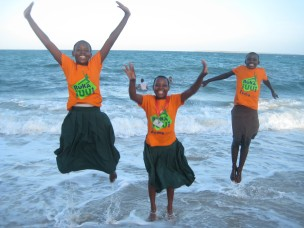
\includegraphics[scale=0.3]{./img/IMG_4778.JPG}}
\end{center}
%Common Challenges and Possible Solutions
\chapter{Common Challenges and Possible Solutions}
We will face a variety of challenges while teaching in Tanzania.  Below are a list of issues volunteers regularly face in their school and ways other volunteers have overcome them. 

\section{Lack of Teachers, especially in the sciences}
Unfortunately, teacher shortage is the most common issue plaguing our school and one we can do little about.  However, there are ways we can compensate for the lack of teachers.

\begin{itemize} 
 \item Try establishing a ``reading room'' in your school with the textbooks you have on hand.  Students can come here to study when a teacher is not present. 
 \item Provide study guides for classes with no teachers.
 \item Choose a student from a higher form to teach forms with no instructor.
 \item Elect student leaders to help with administrative tasks.
\end{itemize}

\section{Poor educational background in students}
Students may enter your school without the ability to read, write, or perform basic mathematical calculations.  Try these tips to overcome poor primary education.

\begin{itemize}
 \item Always teach new Form I students.  Speak to them in English and make learning the language fun for them, so they will continue to study it after the initial orientation course is over. \
 \item Use the first day of a new topic to review material that should have been learned in the past. 
 \item Have academic camps during school holidays to encourage students to re-learn the basics. Math camps have been extremely successful for a number of volunteers.
 \item Create monthly academic competitions between forms, like spelling bees or trivia bowls and offer cash rewards.
 \item Create remedial classes for students who are slower learners.  It allows the teacher to focus on a student's weakness and ways to improve.
 \item Offer free one-on-one or small group tuition. Post your schedule for students to sign up for an hour include name, subject and topic so you can prepare and meet with them in their classrooms.
\end{itemize}

\section{Language barrier}

Its true most of our students don't know English.  But they aren't going to learn it if you teach them in Swahili either.  Try fun and interactive lesson plans that can allow you to teach in English and still convey meaning.\\

See Chapter 7 or the English Teaching Manual for more ideas.

\section{Corporal punishment}
When schools are  hard pressed to find teachers, keeping discipline in a school becomes difficult.  This is why so many schools use corporal punishment; it is quicker to hit a student with a stick than stay after school to administer detention.  Other that the obvious human rights violations, corporal punishment does not fix the core problem: students' behavior. Students fearing a stick means they will only behave when threatened with punishment.  Therefore, when we use corporal punishment we are not teaching our students how to behave and this will result in a disconnect between actions and results for the rest of their life.  Below are the national government regulations regarding corporal punishment:
\begin{enumerate}
\item This regulation may be cited as the National Education Corporal Punishment Regulation, 2002.
\item In these regulations, unless the context otherwise requires: Corporal Punishment means punishment by striking a pupil on his hand or on his normally clothes buttock with a light, flexible stick but excludes striking a child with any other instrument on any other part of the body.
\item Corporal punishment may be administered for serious breaches of school discipline or for grave offenses committed whether inside or outside the school which are deemed by the Head of School to have brought or are capable of bringing the school into disrepute.
\item Corporal punishment shall be reasonable having regard to the gravity of the offense, the age, the sex, and the health of the pupil and shall not exceed 4 strokes on any one occasion.
\item The Head of School in his discretion may himself administer corporal punishment or delegate his authority in writing to all or any member of his staff provided that the member or staff authorized may only act with the Head of School on each occasion when corporal punishment is administered.
\item Female pupils may only receive corporal punishment from female teachers, except where there is no female teacher at the school in which case the Head of School may authorize in writing a male teachers to administer corporal punishment or may himself administer such punishment.
\item All occasions on which corporal punishment is administered shall be recorded in writing in a book kept for the purpose and such record shall state in each instance the name of the pupil, the offense or breach of discipline, the number of strokes and the name of the teacher who administered the punishment. All entries in this book shall be signed by the Head of School.
\item Refusal to accept corporal punishment either by a pupil or by the parent on the pupil's behalf may lead to the exclusion of the pupil in terms of expulsion and exclusion of pupils from schools' regulations made under the provisions of the National Education Act, 2001.
\end{enumerate}

The best way to overcome corporal punishment at your school is to encourage and reward those with good behavior.  For students with poor behavior, you may refer to Chapter 5 for discipline measures and also hold counseling sessions with the students.  Some may be having problems at home or struggling with academic material. Additionally, many bad behaving students are also truants. If a student misses 90 days of school, they are expelled.  Keep track of students attendance and remove those students who do not want to study and are taking away learning opportunities from their peers.
 
\section{Lack of commitment from teachers}
Talk to the teachers at your school to find the cause of their lack of
commitment.  Be realistically optimistic and try to support them in
ways you can.  Avoid being negative.  Share successes and challenges
and encourage other teachers to do the same.

\section{Limited resources}
Use the subject specific manuals to find alternative forms of teaching materials. 

\section{No student support system after school or at home}
Students live at home, in hostels or in ``ghettos".  A ``ghetto" is a
room rented by students whose families live in neighboring villages.
During the school year some students have no support at all.
\begin{itemize}
\item Stimulate parent and community involvement by hosting an event for
them (open house, drama, or talent show).
\item When parents or other villagers are complaining about the state of
local education, explain the roles of PTAs and school boards in
America and how much control parents and community could have in
school systems.
\item Ask students what they do after school, visit their ghettos and host
extracurricular activities or tuition.
\item Start a life skills, peer education or big brother/big sister
program to keep students from negative influences and to give them
confidence and experience to support each other.
\item Take students up on invitations to visit their families.  Our
conversations with parents and relatives about education, America,
coming to Tanzania might inspire a family to support their children in
education.
\item Encourage students to become supportive parents.  Emphasize the
importance of education and the impact of teaching children at a young
age.  Maybe one day students will remember our preaching and their
children will be supported.
\end{itemize}

\section{Lack of student interest to learn}
Teach the students who are interested.  Spend time out of class
getting to know the others.  Most of them do not understand the power
of education.  Some have difficult situations at home, others have
insufficient academic background.
\begin{itemize}
\item At the beginning of each semester teach study skills (note taking, test taking, how to have a group discussion, etc).
\item Provide positive alternatives to academics. Participation in sports, drama clubs, self-reliance projects and life skills programs gives students skills they will be able to use when they have failed school.
\end{itemize}
\section{Teacher training}
Teachers with university degrees tend to get jobs in A Level schools,
Teachers' Colleges or administrative positions.  Other teachers have
certificates to teach in primary school or diplomas to teach secondary
school from 2 years of post-secondary study in Teachers' Colleges.
Part of the education in Teachers' College includes "field" a student
teaching experience in village school.  Schools with insufficient
teachers will hire students who have finished form 6 with Division
3-15 or higher.  Form 6 leavers have possibilities of continuing their
studies and usually work short contracts with the Head of School.\\

There are many opportunities for professional development at work.
Take time to get to know and understand  your colleagues.  Encourage
feedback from your fellow teachers.  Likewise, if you see a weakness,
find an appropriate time and place to offer advice on how to overcome
that weakness.\\

Respect other teachers, even those who have little training or those
with whom you disagree.  It is easy to think of teachers (especially
form six leavers) as incapable of teaching but better to think of them
as potential.  Sharing alternative teaching methods and successes in
the classroom may inspire you and others and make your experience much
more rewarding.

\section{High school fees}
Try setting up a scholarship fund from donors back home. Or reach out to local NGOs who fund education.

\section{Poor School Leadership}
In some instances, your Head of School or other administrators may not be fulfilling their duties. Thankfully, many of us teach in schools with a small teaching staff, which can allow us to enter roles of leadership and compensate for these shortcomings.  Additionally, Peace Corps has been trying to foster relationships between District Education Officers and PCVs.  If your Head of School is not listening to your point of view or violating their role as Head of School, you may seek advice from fellow teachers and possibly consult your DEO.

%Setting Up and Maintaining a Library
\chapter{Setting Up and Maintaining a Library}
It is probable that your school has a variety of textbooks and old donated resource books hidden away in the headmasters office or in the Academic Office.  This books aren't being used because your school probably has no way of managing a system that will ensure books won't be stolen or damaged. \\

Conversely, you may be at a school that already has a library, but it is constantly locked or students never seem to use it.  Have no fear.  There are easy ways to overcome these challenges and get your students reading and using the materials your school already has available. \\
\begin{center}
\setlength\fboxsep{0pt}
\setlength\fboxrule{2pt}
\fbox{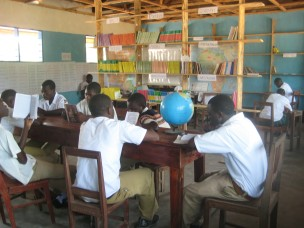
\includegraphics[scale=0.3]{./img/IMG_3883.JPG}}
\end{center}

\section{Steps for Creating a Library}
\begin{enumerate}
\item Collect the books in your school, leaving one copy of each in the Academic office. Ask for book donations through organizations like Read International or Books for Africa.  Your District Education Officer should know about both of these NGOs as they are extremely active in Tanzania and usually consult the DEO before making donations. You will get some outdated material as well as some amazing donations. You could also have businesses donate bookshelves, tables and chairs in exchange for having a business name engraved right on the supplies donated.

\item Ask for monetary donations through your school, PPCP or SPA grants to build tables and shelves.

\item Organize your library once you have enough material. Figure out how you want it displayed and organized. Maybe you want to organize by subject or have a section that is textbooks and another that is reference.  You could also organize by form.  Make sure you get students involved at this stage.

\item Create a catalog system and inventory so you can keep track of which books are where in the library. Try writing the number of books in each subject on the shelf so you can quickly take daily inventory to see what is missing.

\item Take applications for student librarians. Usually one student per form is appropriate. Find students that are passionate about studying but can also stand up to noise makers. Too many can make things complicated.  Develop a set of rules together for the Library.  Can students check out books or are they only allowed to be used in the library? Should students be allowed to bring in bags? How many students can use the library at one time?

\item Develop a monitoring program.  The library can only be used when the teacher or a student librarian is present. Have students sign in and out when they come into the library.  Student librarians should count all the books at the end of each day.  If a book is missing, you know who used the library and when. This way the book can easily be recovered.

\item Encourage the students to use the library.  Schedule library time into the school time table when there is an open period.  Encourage teachers to use it.  Hold class there rather than bring books to class. Hang up students work in the library. Have movie nights there for students who live on or near campus. Try to develop a culture of reading.

\item Look for ways to improve your library.  Be sure to always include Tanzanian staff to create sustainability. 

\end{enumerate}
%Passing NECTA
\chapter{Passing NECTA}
\section{NECTA Overview}

     National Examination for Standard 4, Standard 7, Form 2, Form 4, Form 6 and Teacher Training Colleges are prepared by the The National Examination Council of Tanzania.  The NECTA exams are based on the syllabus prepared by Tanzania Institute of Education, which falls under the administration of the Ministry of Education and Vocational Training. The exams are composed by teachers from secondary schools and other experts who are selected by NECTA. Marking schemes are also prepared by teachers and are discussed and agreed upon before the marking of the exam is begun. \\
      There is one simple reality for all students in Tanzania: the national examinations are the only thing that matters.  This can be a source of tremendous frustration for PCVs.  On one hand we want to teach our students well, but on the other hand we are expected to help them pass their exams.  These goals do not have to be in conflict, though it can often feel as though they are.\\   

      As one PCV recounted, "when I came to Tanzania, I wanted my students to understand chemistry and the world around them...  They did...  And then they all failed their examinations."  The examinations are difficult because they test obscure material, require memorization of very specific details and each subject has a huge amount of content.  As a result, it is nearly impossible for a student to receive a perfect score on any examination.   \\

      This means that PCVs must consider the examinations in almost every lesson they do with their students.  The exams are beatable in the sense that at some point you can cover all possible material, but this is unlikely to happen in village schools because of language issues, lack of teachers over four years and lack of focus from students.  You will have to condense your material in a way that is easy for the students to understand and memorize. 

\section{Lessons for Passing NECTA}
Here are a few questions to ask yourself when planning a lesson:
\begin{itemize}
\item How was this topic tested on past examinations?
\item What definitions must be given?
\item What drawings must be given?
\item What points must be given? (For essay questions, 5-8 points are required)
\item What topic is it paired with for comparison questions? (Ex digestion and respiration)
\item What common mistakes are students going to make?
\item What is the basic strategy for solving any problem similar to this one?
\item What advantages/disadvantages are there for each subtopic? (Ex advantages of angiosperms)
\item What vocabulary must they know?
\item What past content can I include in this new lesson to help the students review?
\end{itemize}

      Ideally, PCVs will spend a lot of time reviewing past examinations before preparing lessons.  It is good to begin from 2001, when the new format for examinations began.  There are NECTA past paper books available at any book store and past exams are also kept by every school.  Once you have reviewed these past examinations, you will get a feel for what kinds of questions they ask.  When you prepare a lesson, always review past NECTA questions on the topic before planning how you will teach it. \\

\section{Divisions} 
      Divisions are the groups used to determine which students go to A-level.  In order to continue on with education, a student must get division one or two.  It is possible for some division three students to continue on to A-level, especially girls and science students.\\   
      The examination system of Tanzania follows the '3 Cs' rule.  This means that if a student in O-level wants to continue on to A-level, they must receive at least a C in all three subjects in their combination.  For example if they want to continue with the PCM combination, they must have received at least a C in physics, chemistry and mathematics.  Grades in other classes are important in calculating their division.  If a student receives division 1 or 2 with a minimum of 3 C's in their desired A-level combination, they are going to be chosen to attend an A-level school. \\

      If you receive an F in mathematics, English, Kiswahili, or civics, you will automatically receive division 3 or below.  English and Civics are very easy to pass, so if a student is going to get division 1 or 2, it is unlikely that they will fail either of these classes.  The trouble is with Kiswahili and mathematics.  Mathematics is a subject that many Tanzanian students struggle with, even though passing (getting 21\%) is possible for even the worst math students.  If you are a math teacher, remember that your students chances of continuing on with their education are greatly influenced by their math grades. \\
      The grades are determined using the following scale (note that a student only needs 21\% to pass any subject):\\

      A 81\%, B 61\%, C 41\%, D 21\%, F 20\% or less\\
      
      The system for determining divisions is simple.  NECTA will take the highest 7 grades and use them to calculate the students division using the following point scale. \\

      A 1 point,  B 2 points, C 3 points, D 4 points, F 5 points \\

      Divisions work like golf, the lower the score, the better the student has done.  Here is a breakdown of divisions by point value (note that the best score is a 7): \\
\begin{flushleft}
Division 1: 7-17 points\\
Division 2: 18-22 points\\
Division 3: 23-25 points\\
Division 4: 26-30 points\\
Division 0: 31+ points, the student has failed the examinations completely\\
\end{flushleft}
 
      In Tanzania, a students future will be determined by the division they get.  This is why it is so important for PCVs to consider the national examinations in everything they do in class.  If you help your students score better on their exams, it can drastically change their options for the future.  The options for various divisions work like this: \\
\begin{flushleft}
Division 1, 2: A-level, lower point totals mean acceptance into better schools\\
Division 3: Some students, especially girls can still go to A-level.  Students taking science combinations have a good chance of continuing if they meet the 3 C minimum, arts students still have a chance though space is limited.  For those who are not accepted, they often end up going to a teachers college to become primary school teachers.\\
Division 4: Police, VETA (vocational schools), nursing, army\\
Division 0: Shamba, machinga\\
\end{flushleft}

\subsection{Form 2 National Exams }
      The Form 2 exams are not particularly important.  They used to prevent students from continuing on the form 3 and 4, but this has since ended.  This means that students do not have any meaningful examinations until their form 4 NECTAs. This can cause problems for PCVs who teach chemistry and physics.  In Form 1 and 2, these subjects are mandatory, but they can be dropped during form 3 and 4.  This means that form 1 and 2 students who know that they will drop these science classes often don't pay attention in class. \\

      There are no divisions for form 2 students.  Instead they just use averages.  The grades are calculated as follows:\\

      A 81\%, B 61\%, C 41\%, D 30\%, F 29\% or below\\
       
\section{Exam Formats and Grading} 

      All examinations for subjects taught by PCVs involve some combination of multiple choice, fill in the blank, matching, essay and math problems.  The grading for much of this is obvious and does not need explanation, however, the math problems and essays do require a bit of explaining.  The information below is targeted towards English and mathematics, but it applies to similar questions in the other subjects as well. 
      
\subsection{NECTA Math Grading} 
      Grading mathematics is very simple.  The number of points a question is worth is generally related to the number of steps involved in solving a problem.  The final answer is only worth 1 point and the rest is split among the work shown to arrive at the answer.  Students must write all of their answers neatly, showing each step clearly for the grader to grade.  Scratch work is written on a separate paper and is not turned in with the exam.  During the national exams, the right side of the paper is used for marking only.  It is a good idea for students to use a ruler to make this space when the are doing exams in school prior to taking the national examinations. This way they get used to leaving this space to the graders.  Writing in this area will result in lower scores. 

      When students are writing on their answer sheets, they do not have to write their answers in order.  It is expected that their answers are clearly marked and written neatly.  As with other classes, all drawings are expected to be drawn in pencil, while everything else is written in ink.  Students are allowed to skip steps in algebraic simplification if they are able to do it correctly. 
\begin{flushleft}
    
\textbf{Section A (60 Marks) }\\
Contains 10 questions worth 6 points each\\
Questions come from any topic from form 1-4\\
 
\textbf{Section B (40 Marks)} \\[20pt]

Contains 6 questions, the student must choose 4 and they are worth 10 points each\\
Topics are only from form 3-4 and the topics are always predictable\\[20pt]

Q11 is linear programming\\
Q12 is statistics\\
Q13 is 3 dimensional shapes and earth as a sphere\\
Q14 is matrices and transformations\\
Q15 is book keeping and accounting\\
Q16 is probability and functions/relations\\[20pt]

Since the questions come from predictable topics, its good to review the easier topics like linear programming, statistics and earth as a sphere with form 4's before their exams.  Since each question is worth 10 points, getting 2 of these correct will almost guarantee that the student passes mathematics\\

\end{flushleft}  
 
\subsection{NECTA Essay Grading} 
  For many new PCVs it can be a bit of a shock to watch a Tanzanian grade an essay.  They grade it in less than thirty seconds and pay little attention to the grammar or spelling.  There is little thought put towards the quality of the argument being expressed.  What is most important is that the essay is easy to mark and that the examples listed are found in the grading scheme.   

      Essays require between 5-8 points supporting their answer.  In the past 5 points were required, but during the 2010 examinations 8 points were required.  This was not announced by NECTA and it is unclear if this will continue.  It is a good idea for teachers to try to give 8 points to their students instead of 5, in case this continues in future examinations. \\

      When grading essays there are a few general guidelines to follow.  All essays are worth 20 points and the grading generally breaks down like this: \\

\subsubsection{Introduction (2 points):}
\begin{itemize}
\item The introduction must contain the definition of the topic being discussed
\item It should contain key participants, theories, or people that are relevant to the topic
\item If it is a question asking for an opinion, they should state very clearly what their opinion is
\item If they are writing an essay where they must imagine that they are someone, it should be done in the voice of that person.  For example if the question asks for a student to write an essay as an Agricultural Extension Officer, its best to begin with something like Dear people, I am in front of you today as your Agricultural Extension Officer to give you advice on how to improve farm yields.
\end{itemize}

\subsubsection{Body (15-16 points)}
\begin{itemize}
\item Contains 5 or 8 points which support their view.  The best points should be written at the beginning, in case they are only grading 5 points.  Its best to try to write 8 unless you know that NECTA will grade only 5.
\item Each point must be its own paragraph.  Most paragraphs consist of only 2-3 sentences.
\item 1 point is given for the point itself.  It should be clear and simple.  Often students underline the point, though this isn't recommended or required.  The first sentence of each body paragraph should just be the point stated with nothing else.  The support comes in the second and third sentences
\item 1 point is given for the explanation and examples found in the second and third sentences.  This can also be given for neat writing and correct paragraph arrangement.  It depends on the grader of the examination.  If it is a 5 point examination, this part is worth 2 points instead of 1, usually split between neatness and support of the point being made.
\item Grammar is not considered unless there are very serious errors or the sentence cannot be understood, even for English exams.  NECTA graders often do not have good enough English to correct these essays.  Also, there are so many errors made by students that grades would be severely affected if grammar and writing quality were considered.
\item Flow is not important.  Students are not expected to use transitional sentences.
\end{itemize}

 
\subsubsection{Conclusion (2-3 points)}
\begin{itemize}
\item Contains a short summary of what you have written
\item Contains the students opinion on the issue of the essay
\item They can begin the conclusion with In my view... or In summary...
\end{itemize}

 Some of these criteria might make an English teacher squirm, but remember that the most important thing is that the essay is easy for the grader to mark.  This format does not exist because the Ministry of Education thinks that this is the ideal way to express ones ideas, but rather it allows them to push through thousands of examinations in a reasonable amount of time.
%Interactive Teaching Ideas
\chapter{Interactive Teaching Ideas}
\section{Biology}
\subsection{Form I}
\subsubsection*{Introduction to Biology}
\begin{itemize}
\item	When teaching fields related to biology, draw picture flashcards, quizzing students on meaning.
\item	Ask students what they think they can use biology for and have them make a short list that can be shared with the rest of the class.
\item	If they are totally ``clueless'' try to bring  in one or two professionals who studied biology as preparation for their career.
\item	Have a plant, human, and insect.  Ask students how we know these things are living.
\item	Ask students to use 5 senses to verbally describe a flame. Use this experiment as example for lab notebook
\item	In groups of 4 students will conduct a series of experiments (Who is the tallest in your group? Who has the highest temperature? Who has the quickest pulse? What is heaviest, rock, pen, or shoe?) using scientific method and lab notebooks to record.
\end{itemize}

\subsubsection{Safety in Our Environment}
\begin{itemize}
\item	Draw or have students draw pictures of common household accidents.
\item	Have students draw the common hazard signs in a laboratory and hang around the classroom..
\item	Act out First Aid procedures in class, making sure students know the name of the injury and how to treat it.
\item	Bring in a First Aid box.  Ask students what is inside and what it is used for.
\end{itemize}

\subsubsection{Health and Immunity}
\begin{itemize}
\item	For manners and hygiene: have students draw pictures of people with good manners and people with bad manners. Same with good hygiene and bad hygiene.
\item Use chalk dust or glitter (beauty shops) to show germs and how easily they can be passed from once person to another. 
\item Have four students link arms to create a wall, showing the body's first line of defense. Have another student, or pathogen, try to break through the line to enter the blood stream.  Then remove one of the students from the first line of defense and have the pathogen enter through that hole.  Two other students will act as white blood cells to try and fight the incoming pathogen.  Be sure students have name cards or sheets of paper to indicate their role in the play.
\item Use activities from the Life Skills Manual, HIV manual, or MoEVT peer teaching book when giving lessons about HIV.
\item Role play ways to say no to sex.
\end{itemize}

\subsubsection{Cell Structure and Organization}
\begin{itemize}
\item Teacher draws the two cells on the board and has students try to place labels on the correct parts of the cells.  Students learned parts of cell in primary school, but in Swahili, so this activity will give them confidence to show what they already know.
\item Have students observe onion cells using a water drop microscope. (Google water drop microscope)
\item Give 8 students a manila card, each saying a different level of organization (atoms, molecules, organelles, cells, tissue, organs, organ systems, organism) Have the class try to arrange the students from smallest to largest to show order of organization.
\end{itemize}

\subsubsection{Classification of Living Things}
\begin{itemize}
\item	Give students cards which they will draw plants and animals they see around them.  Then have them classify based on similarities and differences.
\item Using playing cards, have students group the cards by color (not as specific) and then by suit. (more specific) 
\end{itemize}

\subsection{Form II}
\subsubsection{Classification of Living Things}
\begin{itemize}
\item Bring in yeast, mushroom, and bread mold for students to observe with a magnifying glass and draw.
\item Start the class with a nature walk observing different plants. Ask students what the plants all have in common, leading to the features of Kingdom Plantae.
\end{itemize}

\subsubsection{Nutrition}
\begin{itemize}
\item Begin the class by asking students to call out their favorite foods.  At the end of class, use these foods as examples to classify as carbohydrate, protein, lipid, etc.
\item Show students pictures of different organisms and have them call out if they are heterotrophic or autotrophic.
\item Have students create a menu for the day that is a balanced diet. They must include 6 serving of grain, 3 of milk, 3 of protein, 2 of vegetables, and 2 of fruit.  
\item Draw the digestive system on the board and have students guess the location of certain organs as you teach them using card labels.  You can also write the function of the organ on the back of the cards and review the next lesson reading the function and students calling out the organ.
\item Draw 8 plants on different pieces of paper, one normal and the others suffering from different mineral deficiencies. Have students observe each and compare to the health plant picture.  Ask them what they observe, using their observation to lecture on mineral deficiencies in plants. Quiz students later with the pictures and ask them what mineral is missing and how they know.  
\item	For Photosynthesis, have students draw a real leaf to learn the parts.
\item Remember to do photosynthesis and food test practicals, they are simple and kids love them.
\item Bring in different foods that have been preserved and have students try to guess which method of food preservation was used. Then have students taste a food that was preserved by drying and the same food fresh.  Ask them if they taste the same or different. Explain that this is a negative effect of traditional methods, they change the taste of food.
\end{itemize}

\subsubsection{Balance of Nature}
\begin{itemize}
\item After lecturing on the natural environment, have students race to complete a scavenger hunt.  Write 5 questions on 5 different slips of paper.  When they finish the task of one question, they can get another task. The first group to finish wins. Example questions: draw an example of a secondary consumer, bring the teacher an abiotic thing in the environment, write the definition of an ecosystem, draw an example of a producer, list four reasons we should protect the environment.
\item Break students into small groups and give them pictures of different organisms and a piece of chalk.  Have students first group the organisms by their tropic level, then create a food chain, and finally a food web.  Walk around and observe each group. 
\end{itemize}

\subsubsection{Transport of Materials}
\begin{itemize}
\item Give a few students pieces of paper that say waste, energy.  Have two students acts at blood cell, one handing out cards that say food and oxygen and the other that collects waste and energy.  Explain that our blood transports materials.
\item Spray perfume in the corner of the room and have students raise their hand when they can smell it.  Then have students repeat the exercise, using themselves to represent the particles, starting in one corner of the room and dispersing until they are evenly distributed.
\item Using desks to represent a membrane, have students diffuse from one side to another.  Then show a semi permeable membrane and only let girls pass through.
\item Using colored chalk, draw a large heart and the rest of the circulatory system on the floor.  Have students walk through the circulatory system, stating where they are and where they are going next.
\item Place a few drops of Gentile Violet (purple stain used for surgery, Pharmacy) into water and then place a cut stem of a monocot and dicot into the solution.  After a few hours, make a thin cross section of each and have students observe using a magnifying glass.  They will be able to see the vascular bundles and differentiate between monocots and dicot. 
\end{itemize}

\subsubsection{Gaseous Exchange and Respiration}
\begin{itemize}
\item Have students breath in through their nose only.  Then have them breath through their mouth only.  Compare the two types of breathing and list the benefits of breathing through the nose.
\item Show photos or have students observe different types of organisms and the organs they use for respiration.
\end{itemize}

\subsection{Form III}
\subsubsection{Classification of Living Things}
\begin{itemize}
\item After presenting information about monocots and dicots, give students specimens labeled A, B, C, and D (maize, bean, mango, and cashew) Have them identify kingdom, phylum, class, common name, and two observable features that allowed them to classify the specimen.
\end{itemize}

\subsubsection{Movement}
\begin{itemize}
\item Teacher acts out each form of locomotion and students call out what type. For ciliary use your fingers, for flagellary use a belt as a flagellum, and for muscular, walk.
\item Bring in joints from the butcher to show students different types.
\item Have students grip their bicep, flexing and relaxing their arm to feel the shortening and lengthening of the muscle.
\end{itemize}

\subsubsection{Coordination}
\begin{itemize}
\item	Throw a ball at a student.  Have them then list the steps of nervous coordination from stimulus to response.
\item Break students into small groups. Give each card that says a stimulus on it and have students write the 5 components of nervous coordination that will occur. For example: Seeing a snake. Stimulus: Snake, Receptor: Eyes, Coordinator: Brain and spinal cord, Effector: Leg muscles, Response: Run away! 
\item Have many students stand in a Y shape. One end of the Y is sensory neurons which lead to the brain and then go back down to the other end of the Y which is motor neurons.  Have students send a message (either squeezing hands or saying a word) that starts at the sensory neurons travels up the relay neurons to the brain and then back down to the motor neurons.
\item Measure students reaction time by dropping a meter stick through their open hands. Explain that this is nervous coordination.
\item Draw a large nerve ending, synapse, and dendrite of another nerve on the ground.  Have students act as synaptic transmitters and cross the synapse to send a message.
\item Use dominoes to show threshold, refractory, and all-or-none principle.
\item Role play effects of drugs and ways to say no.
\end{itemize}

\subsubsection{Excretion}
\begin{itemize}
\item Draw a large nephron on the ground with chalk that is big enough for students to walk through. Split the students into groups, giving each group pieces of paper with  the name of different substances on it (water, salt, sugar, blood cells, urea). One by one have the groups walk through the nephron, with different substances either leaving the nephron to go back to the blood or following the nephron all they way through to the bladder. Have two students be sphincter muscles which let the other students out of the bladder.
After all groups have gone, allow students to go one by one, each time getting a different substance and leaving the nephron at a different places. If time allows, you can also introduce the role of ADH by having some students labeled ADH go in and pull water back out of the nephron and into the blood stream. 
\end{itemize}

\subsubsection{Reproduction}
\begin{itemize}
\item Have students match pictures of asexual reproduction with the different methods.
\item Send students outside to collect any flower they like, encourage them to find one that is unique and different. Then have students draw and label their flowers, determining whether they are male, female, or bisexual.
\item Ask students to list all the changes that have occurred in their bodies between Form I and Form III. Explain that these changes are puberty!
\item Draw a large uterus/vagina and penis on the ground. Put the students into groups and give each group a different method of contraception (pills, condom, IUD, spermicide...). In each group, some students will act as sperm, another as and egg and other as the birth control method. Have the class count down (3-2-1 EJACULATE) and the sperms run out of the testes and try to get to the eggs. The contraceptive students prevent the pregnancy from occurring. For example, a condom would create a barrier to prevent the sperm from entering the vagina, an IUD would allow the sperm to meet the egg but then push the egg out so it cant implant, pills would take the egg away, tubal litigation would cut the path so the egg cant pass and spermicide would kill the sperm.
\item Mitosis and meiosis can be acted out in a song and dance. Then students can remember the stages in the song form and the actions that go along with each stage.
\end{itemize}

\subsubsection{Regulation}
\begin{itemize}
\item Ask students to act as if they are very cold.  Note what they do (shiver, rub their arms, etc.) Then have students behave as if they were in a very hot environment, and note their behavior (sweat, fan themselves, etc.) 
\end{itemize}

\subsection{Form IV}
\subsubsection{Growth}
\begin{itemize}
\item	Plant bean seeds in water bottles and stagger them so you can show the class stages of growth or have students grow their own.
\item	Using matches, string, and paper circles, students act out the stages of Mitosis
\item	Choose 9 students, 2 are DNA, 1 is mRNA, 1 is a ribosome, and 5 are amino acids. Draw a circle on the ground to represent the nucleus, where the DNA will stand.  Each amino acid has a number, 1-5 on them.  DNA will create a combination of the numbers 1-5 and write on a piece of paper.  The mRNA enters the nucleus and makes a copy of this combination and carries it to the ribosome.  The ribosome then arranges the amino acids accordingly.  Protein Synthesis!
\end{itemize}

\subsubsection{Genetics}
\begin{itemize}
\item Using post-it notes, write different bases (A,T,G,C) on a few.  Draw two lines on the board and add a few bases to the left strand.  Have students place corresponding bases on the other strand and then write the genetic code for that DNA strand.  These post-its can be used later to show different types of mutations.
\item Have students race to complete Punnet Square questions.
\item Have students measure their height, hand span, number of boy and girls, and those who can and can not roll their tongue.  Graph each to show continuous and discontinuous variation.
\item Break students into groups. Each group will get two piles of seeds. The first pile will be all maize seeds (X chromosomes)-this the mother-and the second will be half maize and have beans (half X and half Y)-this is the father. Students should close their eyes and draw one seed from each pile. If the get two maize seeds, it is a baby girl. An X and a Y is a baby boy. This can be extending with another trait like albinism or eye color where a dominant and a recessive trait is involved.
Similarly this activity can be done with coins which have taped letter (X and Y or B and b) on either side. Students should choose from the pile or flip the coins many times and then record the percentage of each phenotype and genotype observed. The teacher can compile the data from the whole class.
\item For variation, have two students stand in front and have the class give all of the differences between them. Then sort these differences into inherited or acquired differences and continuous or discontinuous.
\end{itemize}

\subsubsection{Classification of Living Things}
\begin{itemize}
\item To begin topic, have students race to write as many animals as possible in 3 minutes.
\item	Using hand drawn pictures of organisms on manila paper, teacher uses them like flashcards, quizzing students on kingdom, phylum, class, and three features of each.
\item	Students ask 20 questions to get to an organism the teacher is thinking of.  For example, is it in Kingdom Animalia? Does it have wings? Is it warm blooded? 
\item Have students create Public Service Announcement on how to prevent getting Tapeworm.
\item Have students complete a Venn Diagram showing the differences between Nematoda and Annelida.
\item Show students an x-ray or skeleton to prove that humans do have a tail and belong to Phylum Chordata.
\item Break students into small groups.  Each group draws a different mammal (bat, cow, human, dog, lion, goat, cat) Ask students to call out what they see in their picture and write these features on the board.  Circle the common features that all organisms share (teeth, hair, mammary glands).
\end{itemize}

\subsubsection{Evolution}
\begin{itemize}
\item Have students come together and then explode apart to show the Big Bang Theory.
\item Show students a fossil of a snake when they had legs (internet) then ask students if snakes have legs now. 
\end{itemize}

\subsubsection{HIV, AIDS, and STDs}
\begin{itemize}
\item Use lessons from the Life Skills Manual, articles from FEMA, and guest speakers to teach students about HIV.
\end{itemize}
%===================================================================================================
\section{Chemistry}
\subsection{Form I}
\subsubsection{First Aid}
\begin{itemize}
\item	Role play injuries and have students treat each other.
\item	Build first aid kits with locally available resources
\end{itemize}

\subsubsection{Chemistry Laboratory}
\begin{itemize}
\item	Have students write the name of lab apparatus on their back, then ask other students yes or no questions to figure out what apparatus they are. ``Am I made of glass? Do I hold liquid?''
\item Draw a picture of the set up on the board and pass out pieces of paper with the names of all the apparatus. Have students place their label on the apparatus in the picture. 
\end{itemize}

\subsubsection{Fire Fighting}
\begin{itemize}
\item	Students can collect different fire starting material and then sort.
\item Teacher pretend to light self on fire/class on fire using different materials (i.e. first ``light'' clothes on fire, then spill ``petrol'' then have an electric fire.) The fire can be a piece of paper with tape on it that is colored and says ``FIRE!''. The students should use materials in the class (water, sand, blanket) to ``put out the fire'' and save the teacher.
\end{itemize}

\subsubsection{Scientific Method}
\begin{itemize}
\item	For observation, light a ``candle'' that is actually made of a potato and a nut for the wick. Have students write observations about the candle and then eat it - throw them for a loop. Discuss difference between observation and inference.
\end{itemize}

\subsubsection{States of Matter}
\begin{itemize}
\item	Bring in water, a rock, and a balloon and ask students to classify each into a state.
\item	Write states of matter on the board.  Then hand students cards reading ``evaporation, condensation.''  Students place cards where they see fit, other students correct as needed.
\item	Have students lock arms to try and represent the different states of matter. Solid is when the students have interlocked elbows, liquid is when they are holding hands, and gas is no holding at all.
\item	Alternatively, have students act out solid liquid and gas by standing close together (solid), walking around in a small area (liquid) and running around (gas). This might be best as an outside activity. Students one by one leaving the liquid state and running around outside of it as vapor can to show evaporation.
\end{itemize}

\subsection{Form II}
\subsubsection{The Periodic Table}
\begin{itemize}
\item	Teacher draws blank periodic table on the board.  Students are given elements and try to place in the table.
\item	``Build'' atoms on the desk with 2 different color beans and corn for protons, neutrons, and electrons. Show different isotopes.
\item	Make cards with the information about the first 20 elements (mass number, appearance, s/l/g, etc.) and have students arrange them according to mass and properties. Guide them to group them into columns with similar properties. They should arrange the elements in the same way as Mendel did.  
\end{itemize}

\subsubsection{Water}
\begin{itemize}
\item	Write the word water in the middle of the board and have students brainstorm everything they know about water. Make a giant mind map. Alternatively have students make mind maps in groups.
\item Have different parts of the room labeled as the different natural sources of water (rain, river, lake, ocean, cloud, glacier...) at each place have a die which can be rolled to tell a student where to go next (some sides of the die will say ``stay''-for example for the ocean 4 sides of the die will say stay and two sides will say ``clouds''). Have students go around the class from place to place and record each place they went. After the activity, have students write stories about a ``day in the life of water molecule''. Where did they go and what did they do?
\end{itemize}

\subsubsection{Oxygen / Hydrogen}
\begin{itemize}
\item Have students draw pictures to represent the different uses of oxygen and hydrogen.
\item Set up or draw the apparatus needed for production of hydrogen and oxygen but do it with many mistakes (e.g. have the gas jar upside down, don't put the water in the trough, forget to attach the delivery tube...). Have students correct all of the mistakes so that the set up is correct.

\end{itemize}

\subsubsection{Oxidative States}
\begin{itemize}
\item	If potassium permanganate is available a dilute solution can be made. Add some sodium hydroxide and put a drop on a piece of filter paper. The color will change from purple to green to brown to pink/colorless as the manganese is reduced by the cellulose in the paper. Explain that the different colors are caused by the different oxidation states of manganese.
\end{itemize}

\subsubsection{Nomenclature}
\begin{itemize}
\item	Assign students elements, and then write the name of the molecule on the board, The students then must try to find the right combination of ``atoms'' to form the molecule. 
\end{itemize}

\subsubsection{Electrovalent Bonding}
\begin{itemize}
\item	Have a boy(+ metal) and girl(- non metal) act as an ionic bond, explaining its like marriage, the boy gives a ring (charge) to the girl and they are linked.  Then have two girls (halogens) act as covalent bond, sharing and supporting each other equally as friends.
\end{itemize}

\subsection{Form III}
\subsubsection{Introduction to Reactions}
\begin{itemize}
\item	Give demonstrations of all the different reactions as they are introduced: double decomposition (ppt between  \ce{Na2CO3} and \ce{CuSO4}), replacement (steel wool dipped in \ce{CuSO4}), combustion (burn paper), combination (heat copper and sulphur), decomposition (\ce{H2O2}=\ce{H2O}+\ce{O2}) 
\end{itemize}

\subsubsection{Balancing Equations}
\begin{itemize}
\item Have students act out the molecules in a reaction. For example, for the decomposition of hydrogen peroxide, have two student be hydrogen and two be oxygen in hydrogen peroxide. Then tell the student to decompose to water and oxygen molecule. They will see that there are not enough oxygens present to do this, so they must double the initial amount of hydrogen peroxide. This is balancing an equation. Alternatively, this can be done in groups using models like fruit and toothpicks.
\end{itemize}

\subsubsection{Hard Water}
\begin{itemize}
\item Give students two tubes/bottles/beakers with water. One should be normal water and the other one hard water containing magnesium sulfate (Epsom salts). Have them determine which water is hard and which water is soft by adding the soap and shaking.
\item Ask students to wash their hands with soap (not
detergent) in hard and soft water.  In separate water bottles mix hard
water+soap, soft water + soap then shake.  Use a third bottle with
boiled temporary hard water to show temporary hardness.
\end{itemize}

\subsubsection{Volumetric Analysis}
\begin{itemize}
\item	In introduction to titration put some pictures of ``husbands/wives'' just outside the classroom door. Tell the class that there are some people who have come to find wife's but you don't remember how many of them there are. Send the girls out one-by-one until one comes back because there is no husband for her. Ask the class how many husbands were outside. This is titration.
You could also add a variation that one wife (acid) can have two husbands (bases) to demonstrate a titration with sulphuric acid.
\end{itemize}


%===================================================================================================
\section{Physics}
\subsection{Form I}
\subsubsection{Introduction to Physics}
\begin{itemize}
\item	Go outside. Walk around and ask students to point out different things that they think are related to physics. Since everything is fairly easily relatable to physics as long, as the students participate, it is a good way to show how applicable physics is in the real world. 
\item	And just be enthusiastic... its contagious. 
\end{itemize}

\subsubsection{Introduction to Laboratory Practice}
\begin{itemize}
\item	Put the class into groups. Give each group a piece of paper with different safety issues in the laboratory written on it.  Have each group put together a skit or song to relay the message to the rest of the class. 
\end{itemize}

\subsubsection{Measurement}
\begin{itemize}
\item	Rotating stations. Each station with question or two (measure the volume of this box, the length of this pen, which bottle has a larger volume, which rock has a larger mass... etc) If you don't have any measuring equipment, make some of your own...a ruler can be made with paper and pen, half of a water bottle as a beaker etc. 
\item	Play jeopardy with conversion questions. If the students cannot convert from km to mm it will be a problem for all physics Forms. One of the most important parts about physics is understanding unit conversion..so make it fun
\end{itemize}

\subsubsection{Force}
\begin{itemize}
\item	Have students stand in a very tight circle front to back. At the same time instruct them all to sit down. If they do it correctly they should be able to each sit on the lap of the student behind them. Its hilarious to watch, and there are forces all over the place. Like many of my suggestions however, more enjoyable than educational. 
\end{itemize}

\subsubsection{Archimedes Principle and Law of Flotation}
\begin{itemize}
\item	For flotation... you can have the students each bring in something they believe will float. Or if just bring in a variety of objects with different densities and have the students hypothesize which they think will float. Then have the students test each. 
\item	Have students form groups. Tell the students to try and build a boat (or just something that floats) and whichever groups boat can support the most weight is rewarded. 
\end{itemize}

\subsubsection{Structures and Properties of Matter}
\begin{itemize}
\item	Have students make a circle, maybe 10 feet in diameter. First show solid by filling the circle with blindfolded students. Tell them every time they touch another student they are to change direction. Since they are tightly packed in a solid, discuss the movement as vibration. Next remove most of the students. Leave, maybe 10 inside. They will be able to move more freely but will still interact. Lastly leave only two or three students to show a gas.  
\end{itemize}

\subsubsection{Pressure}
\begin{itemize}
\item	Use everyday situations. For example, the reason people sometimes put a khanga on their head when they carry a bucket full of water is to decrease the pressure on the top of their head. 
\item	I tried to do a bucket-with-water-on-head relay race using like 15 different teams. This taught them all very little about pressure, but from time to time having a bit of fun will do wonders in the classroom
\end{itemize}

\subsubsection{Work, Energy, and Power}
\begin{itemize}
\item	Put students into groups. Each group will have an object of known mass and they will be required to move that object a certain distance. I set up the activity so that each group would do the same amount of Work (those will small objects would have to go a larger distance, heavy objects not as far). And also ask them to record the amount of time it took to move the object. Then have the groups calculate and compare Work done and Power. 
\end{itemize}

\subsection{Form II}
\subsubsection{Static Electricity}
\begin{itemize}
\item	Visual Demonstration: Take a plastic bag with no holes in it, fill it with air, and close your fist around it making it into a make shift balloon. Rub the bag on your arm or head to electrify the bag.  Use the electrified bag to pick up small scraps of paper you have sprinkled on the table in front of you. 
\item	Static electricity can be difficult for students since the forces are invisible to the naked eye. The rubbing of the bag shows how a body can be electrified by ``rubbing'' ... and the paper scraps jumping onto the bag shows ``induction''
\end{itemize}

\subsubsection{Current Electricity}
\begin{itemize}
\item	Teacher draws a circuit on a piece of paper and then cuts it up to make a puzzle.  Students have to rearrange the pieces to make a circuit.
\item	To build off this...flash lights are easy to find... take a flash light apart, and use the labels used in the previous example. Have the students match the labels to the actual parts because it is very helpful to see what each piece looks like.
\end{itemize}

\subsubsection{Magnetism}
\begin{itemize}
\item	A compass can be made using the bottom of a water bottle, and floating a magnetized needle in the water. This tool can be used to show north and south and if you can find a magnet, you can use it to show the direction of magnetic field lines. 
\end{itemize}

\subsubsection{Forces in Equilibrium}
\begin{itemize}
\item	Find your own mass... see if there are any students who know how much they weigh. If not make the demonstration ``find the mass of a student''. Using a teeter-totter (easily made with a strong piece of wood or metal and something for it to teeter on) find the position of equilibrium between you and the student.  Since $W_{1}X_{1} = W_{2}X_{2}$, and both distances ($X_{1}$ and $X_{2}$) are easily measured, you can find the unknown weight. Hooray for demonstrations
\end{itemize}

\subsubsection{Simple Mechanics}
\begin{itemize}
\item	Find a sturdy piece of timber (sturdy enough to support the weight of a student) and elevate one side of it. Have the student sit close to the elevated side and have the other students feel how easy it is to move him (teaches mechanical advantage). Then put the student of the far end of the stick and have the other students try to lift him putting effort in the middle of the piece of wood. This does a good job of showing 2nd and 3rd class levers.
\item	For 1st class, make a teeter-totter... be creative, you can do it. Show that if the load arm is short and the effort arm is long, you can support a lot more than just your own weight.
\end{itemize}

\subsubsection{Motion in Straight Line}
\begin{itemize}
\item	Another one that is more fun than educational... but that's because I like fun. Take the students to a big open area and have some kind of race (I went with wheelbarrow races and crab walk races) and have those not racing measuring the racers' velocities.
\end{itemize}

\subsubsection{Newton's Laws of Motion}
\begin{itemize}
\item	For Newton's first law: use a bottle, playing card and coin.  Flick the card from between the coin and bottle.  The coin doesn't move because there is no force applied to the coin.  
\end{itemize}

\subsubsection{Sustainable Energy Sources}
\begin{itemize}
\item	This is a tough topic for Form II since they will not learn about generators until Form IV.  But if you construct a small fan or a water wheel (again be creative, both are very doable with simple African resources) use them to show how wind and moving water can turn the wheels. From this motion it is easier I have found for students to see the relationship between natural resources (wind or water) and energy. 
\item	Solar energy can be shown with two bottles containing water, one left in the sun, one kept in the shade. The two will have different temperatures after not too long.
\end{itemize}

\subsection{Form III}
 \subsubsection{Application of Vectors}
\begin{itemize}
\item	Vector problems require practice practice practice. So, rather than just sit and do problems on the board, play a game or have a competition. For example, put students into teams and ask 10 or so vector questions. Working in teams can help the students feel more comfortable which will help to build confidence. At the end collect all the solutions and give the winning team some sort of reward. 
\item	Or, have just two teams. Give one team a chance to solve a problem. Team two will then have a chance to challenge to correct anything they believe to be an error. Go back and forth giving points for correct answers. Make sure the same students do not answer every single question for this game.
\end{itemize}


 \subsubsection{Optical Instruments}
\begin{itemize}
\item	Have students make a microscope using  clear hard plastic with a small hole, a drop of water, and a light source.
\item	Spoons are great tools. They can show both convex and concave mirrors. 
\end{itemize}

 \subsubsection{Thermal Expansion}
\begin{itemize}
\item	Put a sealed bottle containing warm water in class. Ask students to predict what will happen to the shape of the bottle as the water and air cools. Notice the bottle contracts (this may take more than just 80 minutes)
\item	By a balloon and put it on a bottle, put bottle in hot water and observe its rapid inflation... if you have ice water balloon will inflate inside the bottle which is awesome too
\end{itemize}

 \subsubsection{Transfer of Thermal Energy}
\begin{itemize}
\item	Bring in your jiko... show how that even though the mkaa is not in direct contact with the pot that the water will still boil (and the boiling water is a good example of convection). Also if your room is enclosed the temperature in the room will inevitably go up as well. Lots of thermal energy transfer going on here. 
\end{itemize}

 
\subsection{Form IV}
 \subsubsection{Waves}
\begin{itemize}
\item	For transverse: show very simply using a string
\item	For longitudinal I like to bring like ten students to the front and line them up a little less than an arms length a part. Tell them to close their eyes and push the one at the back of the line and observe. If you don't feel comfortable pushing your students, no problem I am sure there are plenty of other ways... this one makes me chuckle though, and does produce an excellent longitudinal wave. 
\item	For sounds waves/echoes/reverberations etc... most of the buildings and rooms are made of concrete. I find these perfect to let students explore their lung capacity and make some noise. Educational and therapeutic. 
\end{itemize}

 \subsubsection{Radioactivity}
\begin{itemize}
\item	Have students be electrons, neutrons or protons and act out beta, gamma, and alpha decay. Make sure you are not just telling them what to do though, have them figure out which particles should come and go on by themselves. 
\end{itemize}

 \subsubsection{Elementary Astronomy}
\begin{itemize}
\item	Have students come up with their own mnemonic devices to remember the planets. Then go through all the ideas and vote on a victor. This technique can be used for remembering things in certain orders really well because the student comes up with their own, and then hears 30-60 other mnemonic devices all with the same letter orders. 
\item	Give each student a fact that relates to a planet (or moon). Stick the names of those planets or moons on the wall around the room and have students try to match their fact with their planet or moon. 
\end{itemize}

%===================================================================================================
\section{Mathematics}
\subsection{Form I}
\subsubsection{Numbers}
\begin{itemize}
\item	Salama Says. Students act out points, lines, and angles using their arms.  
\item	Multiplication flashcards. Many Form I students don't know them and they are a good way to open the year.  
\item	Draw a number line on the ground.  Hand students different numbers on card paper and have them place themselves on the number line.  Emphasis decimals and fractions.
\end{itemize}

\subsubsection{Fractions, Decimals, and Percentages}
\begin{itemize}
\item  Use an orange or tangerine slices to show fractions to the students.
\end{itemize}

\subsubsection{Measurements}
\begin{itemize}
\item Have students use string, yard sticks, or rules to measure each other and plot on a graph.
\end{itemize}

\subsubsection{Geometry}
\begin{itemize}
\item Geoboards are a great way to teach geometry.  Consult the Math Specific Manual for more information.
\end{itemize}

\subsection{Form III}
\subsubsection{Relations}
\begin{itemize}
\item	Use dice or dominoes for sets; use practical examples of sets: husband and wife, teacher and student, etc. 
\end{itemize}

\subsubsection{Functions}
\begin{itemize}
\item	Use coordinate chart drawn on seed bag for students to stick coordinate points; Use of tables is essential and sometimes the students need many points to understand graphing; use geoboard to demonstrate functions.
\end{itemize}

\subsubsection{Statistics}
\begin{itemize}
\item	use little data and demonstrate mean, median, mode;
\item	have students gather and graph ages of 20 students; then find mean, median, mode              
\end{itemize}

\subsubsection{Rates and Variations}
\begin{itemize}
\item	Demonstrate 2:3:5 so give blocks, sticks, etc in that ratio;  Use many practical examples of direct and inverse variations; have students give examples since this will show real comprehension
\end{itemize}

\subsubsection{Sequences and Series}
\begin{itemize}
\item	Group work on Sequence and series; list the numbers of sequence to prove sum, etc.  Translate the question into meaningful math phrases or equations like 4th term is 10+ 2nd term; etc.
\end{itemize}

\subsubsection{Circle Theorems}
\begin{itemize}
\item	Cut out circles for different theorems to show and demonstrate to students; also have students draw what the questions states, in this way the students translates words into the circle picture to solve the question
\end{itemize}

\subsubsection{Earth as a Sphere}
\begin{itemize}
\item	Brought 3 globes to class so students can see latitude and longitude; solve problems as latitude and longitude change
\end{itemize}

\subsubsection{Statistics}
\begin{itemize}
\item	Had students at board to do cash flow, trial balance and balance sheet; demonstrate the ins and outs of accounting or cash flow
\end{itemize}

\section{English}
See the English Teaching Manual

%Appendix: Education Competencies
\chapter{Appendix: Education Competencies}
\section{Education Sector Competencies}
\subsection*{Technical Competency 1: Effectively teach Tanzanian students}

\subsubsection*{Specific Competency 1.1: PCVs will develop critical thinking, creative thinking, and problem solving skills among students}

Learning Objectives
\begin{enumerate}
\item On the final written technical exam, each PCT will explain the acronym SCALE and list down at least five specific methods for promoting critical thinking, creativity, and / or problem solving skills among students, as described in the technical training manual.

\item Throughout internship teaching, each PCT will prepare at least ten
lesson plans that promote critical thinking, creativity, and problem
solving through the use of the SCALE paradigm, as evidenced by the
Continuous Lesson Preparation and Reflection assignment.

\item  Throughout internship teaching, each PCT will consistently demonstrate use of techniques promoting critical thinking, creativity, and /
or problem solving skills among students, as evidenced by feedback on
the Internship Teaching Evaluation Rubric.
\end{enumerate}

\subsubsection*{Specific Competency 1.2: PCVs will improve subject
content understanding among students to increase their
opportunities for continued education.}

Learning Objectives
\begin{enumerate}
\item On the final written technical exam, each PCT will accurately describe
the structure of the Tanzanian education system, educational pathways
for students, and the nature of formal assessments, as described by the
technical training manual.
\item Throughout internship teaching, each PCT will prepare a scheme of
work and at least ten lesson plans that both specifically address syllabus content and past questions from NECTA exams, according to the
standards of the technical training manual and evidenced through the
Continuous Lesson Preparation and Reflection assignment.
\item Throughout internship teaching, each PCT will consistently demonstrate effective classroom management and gender inclusive strategies as described in the technical training manual and evidenced by the
Internship Teaching Evaluation Rubric.
\item Throughout internship teaching, each PCT will consistently demonstrate use of formal and informal classroom assessments, as described in the technical training manual and evidenced by the Internship Teaching Evaluation Rubric.
\end{enumerate}

\subsubsection*{Specific Competency 1.3: PCVs will promote English
comprehension, communication, and use among students}

Learning Objectives
\begin{enumerate}
\item On the final written technical exam, each PCT will list down at least
three methods for promoting English use among students, as described
in the technical training manual.

\item Throughout internship teaching, each PCT will demonstrate use of
level-appropriate English in classroom teaching, as evidenced by the
Internship Teaching Evaluation Rubric.

\item Throughout internship teaching, each PCT will demonstrate consistent use of English in PCT-student interactions, as evidenced by LCF
observation.
\end{enumerate}

\subsubsection*{Specific Competency 1.4: PCVs will develop life skills among students}

Learning Objectives
\begin{enumerate}
\item On the final written technical exam, each PCT will demonstrate knowledge of HIV/AIDS statistics and list down at least three ways of incorporating HIV/AIDS and/or Life Skill content into classroom teaching,
as described in the technical training manual.
\end{enumerate}

\subsection*{Technical Competency 2: Collaborate with Tanzanian teachers}

\subsubsection*{Specific Competency 2.1: PCVs and Tanzanian teachers
will collaborate to increase their subject specific technical skills}

Learning Objectives
\begin{enumerate}
\item At IST, PCVs will use needs assessment, facilitation skills, and quality
tools, to organize, analyse and discuss data with Tanzanian teachers.
\end{enumerate}

\subsubsection*{Specific Competency 2.2: PCV and TZ teachers will collaborate to increase their capacity to develop lessons
that foster critical thinking, creativity, and problem
solving.}

Learning Objectives
\begin{enumerate}
\item On the final written technical exam, each PCT will describe the process
and content of pre-service teacher training, the current in-service training programs, and the modalities through which Tanzanian teachers
may pursue additional training, as described in the technical training
manual.

\item During micro-teaching, each PCT will demonstrate giving and receiving feedback through the Lesson Study process, as evidenced by LCF
observation.

\item During IST, each PCV will engage in the Lesson Study process with
counterpart teachers according to the parameters of the IST Lesson
Study training session.
\end{enumerate}

\subsubsection*{Specific Competency 2.3: PCVs will promote English
comprehension, communication, and use among Tanzanian teachers}

Learning Objectives
\begin{enumerate}
\item PCV will speak level-appropriate English is a way that clear and understandable to fellow teachers, as evaluated by LCF observation.

\item Throughout internship teaching, each PCT will promote and model the
use of English during interactions with fellow teachers, as evidenced by
LCF observation.

\item PCV will encourage, correct, and support English speaking in Tanzanian teachers, as evaluated by LCF observation.
\end{enumerate}

\subsubsection*{Specific Competency 2.4: PCVs will promote Life Skills,
malaria, and HIV/AIDS awareness among Tanzanian
teachers}

Learning Objectives
\begin{enumerate}
\item At the end of IST, each PCV will be able to informally discuss topics of
HIV, Life Skills, and malaria with fellow teachers in the manner taught
in the IST peer education training.

\item During IST, a PCV will demonstrate active listening skills while recommending testing and treatment options as well as other assistance
for people living with HIV, as evidenced by performance in the Active
Listening Training Role Play exercise.
\end{enumerate}

\subsection*{Technical Competency 3: Engage with Communities}
\subsection*{Specific Competency 3.1: PCVs will involve communities and schools in participatory analysis for community
action}

Learning Objectives
\begin{enumerate}
\item On the final written technical exam, each PCT will accurately describe the structure of the Tanzanian schools and community administration,
as described in the technical training manual.
\item During the session on PACA tools, PCTs will implement PACA tools in
their internship schools, as described in the Peace Corps PACA manual.
\item Before IST, each PCV will use PACA tools to conduct a preliminary
needs assessment in their schools, as evidenced by the School Situational Analysis reporting submitted to APCDs.
\end{enumerate}

\subsubsection*{Specific Competency 3.2: PCVs will work with schools
and communities to develop sustainable teaching and
learning resources}

Learning Objectives
\begin{enumerate}
\item At the end of IST, each PCV will develop with a counterpart a teaching
and learning resource enhancement plan, to the standards described in
the IST technical training materials.

\item During IST, each PCV will learn subject-specific technical skills for
the use of locally available materials in the development of teaching
and learning resources, to the standard described in the IST technical
training materials.

\item Throughout internship teaching, each PCT will consistently incorporate locally available materials as teaching and learning resources, as
evidenced by the Internship Teaching Evaluation Rubric.
\end{enumerate}

\end{document}